%% LyX 2.3.0 created this file.  For more info, see http://www.lyx.org/.
%% Do not edit unless you really know what you are doing.
\documentclass[oneside,english]{book}
\usepackage[T1]{fontenc}
\usepackage[latin9]{inputenc}
\setcounter{secnumdepth}{3}
\setcounter{tocdepth}{3}
\usepackage{array}
\usepackage{float}
\usepackage{textcomp}
\usepackage{multirow}
\usepackage{amsmath}
\usepackage{graphicx}

\makeatletter

%%%%%%%%%%%%%%%%%%%%%%%%%%%%%% LyX specific LaTeX commands.
%% Because html converters don't know tabularnewline
\providecommand{\tabularnewline}{\\}
%% A simple dot to overcome graphicx limitations
\newcommand{\lyxdot}{.}

\floatstyle{ruled}
\newfloat{algorithm}{tbp}{loa}[chapter]
\providecommand{\algorithmname}{Algorithm}
\floatname{algorithm}{\protect\algorithmname}

\makeatother

\usepackage{babel}
\usepackage{listings}
\renewcommand{\lstlistingname}{Listing}

\begin{document}
\begin{titlepage} 
	\begin{center}
  
		
\includegraphics[scale=1]{./04.ListaFiguras/logo.png} %
		\vfill
		\vfill
		\hrulefill
		\vfill
		\vfill
		
			{\huge \bfseries A Study of Multi-objective Evolutionary Algorithms applied to 
					Routing and Spectrum Assignment in EON networks}\\[0.4cm] % Thesis title
		\vfill
		\hrulefill
		\vfill
		\vfill

		\large \textit{MAESTRIA EN CIENCIAS DE LA COMPUTACION}\\[0.3cm] 
		\large \textit{TRABAJO FINAL DE MAESTRIA}\\[0.3cm]    

		\vfill 
		\begin{minipage}{0.4\textwidth} 
			\begin{center} \large 
				\emph{Autor:}\\ {Carmelo Luis Fretes Colman} 
			\end{center} 
		\end{minipage}

		\vfill

		\begin{minipage}{0.4\textwidth} 
			\begin{center} \large 
				\emph{Tutor:} \\ {D.Sc. Diego P. Pinto-Roa} \\ 
			\end{center} 
		\end{minipage}\\[3cm]  

		\textsc{\LARGE San Lorenzo - Paraguay}\\[1.5cm] 
		\textsc{\LARGE 2018}\\[1.5cm]   
		
		\vfill 
	\end{center} 
\end{titlepage}

\pagestyle{empty}

\begin{center}
\textbf{\textit{Dedicatoria}}
\par\end{center}
\begin{quotation}
\textit{A mi hija, mi inspiraci�n.}

\textit{A mis padres y mis suegros.}
\begin{flushright}
\textit{Carmelo Fretes}
\par\end{flushright}
\end{quotation}



\begin{center}
\textbf{\textit{Agradecimientos}}
\par\end{center}
\begin{quotation}
A mi familia, a mi tutor, por la gu�a, paciencia y la motivaci�n durante
todo el proceso de investigaci�n y la elaboraci�n de esta tesis.

A mis compa�eros de trabajo y amigos por las colaboraciones.
\end{quotation}



\tableofcontents{}

The increase in network traffic and the need to increase the capacity
and performance of the stretches of transport networks, born the interest
in elastic networks. At present, the optical transport technology
used in optical networks is Wavelength Division Multiplexing (WDM);
this technology has the capacity to transport, route and assign (Routing
Wavelength Assigment) multiple channels in a same fiber based on carriers
of different wavelengths. This implies that channels with little demand
than the maximum supported, underutilize resources. Therefore, the
flexibility of the spectral grid would be the solution, allowing transmission,
routing and allocation. (RSA - Rounting and Spectrum Allocation) of
channels with variable bandwidth that adjust to the demand. In WDM
networks, routing planning and wavelength allocation algorithms (RWA)
search for a physical route through the network and assign a wavelength
for transport, the selection of that wavelength is conditioned to
be the same during the route of the physical route, this condition
is called a condition of continuity. In the elastic optical networks,
the algorithms of routing planning and spectrum allocation (RSA),
apart from the aforementioned condition, there is a new condition,
which is the condition of contiguity in the spectrum. This condition
stipulates that the frequencies slots that occupy each channel must
be together in the spectrum. The RSA problem can be attacked as routing
and spectrum allocation together. With this approach to the RSA problem,
the greatest difficulty that arises is the large number of conditions
posed by the problem; a greater computational complexity is introduced
when calculating the optimal path for each request while optimizing
the spectrum allocation. The heuristic proposed in this paper is a
multiobjective evolutionary algorithm that determines a set of optimal
Pareto solutions that are not dominated with respect to the others
for the RSA problem. The different tests performed with this algorithm
show promising results with respect to the paper presented in {[}16{]}. 



\chapter{INTRODUCTION}

\section{MOTIVATION }

The emergence of the interest in elastic optical networks (EON) comes
from the constant increase in network traffic and the need to increase
the capacity and performance of the sections in the transmission networks.
At present, the transport technology used in optical networks is wavelength
multiplexing (WDM). This technology is capable of transporting multiple
channels in the same fiber, based on carriers of different wavelengths.
The implication of this technology is that channels that have a reduced
demand to the maximum supported by the granularity imposed, underutilized
resources; given this and because network traffic will be highly heterogeneous,
the flexibility in the provision of optical network resources is a
challenge. A major change in the architecture of EON is the replacement
of the fixed grid with a new flexible grid. The ITU-T is working on
the revision of a new G.694.1 standard \cite{huang2012}. 

The calculating of an elastic optical routing has two parts: (a) optical
routing operations (R), where calculations of the route between the
originating node and the destination are made through a network topology,
and, (b) selection of spectral resources on optical fibers (spectrum
assignment, SA). 

In WDM networks, the algorithms for routing planning and wavelength
assignment seek a physical route through the network and assign a
wavelength for the transport of that channel. The selection of that
wavelength is conditioned to be the same during the route of the physical
route, so that in this way it is not necessary to use wavelength converters
in any jump. This condition is called a continuity condition (continuity
constraint). In EON, apart from this condition, there is a new condition
that is that of contiguity in the spectrum (contiguity constraint).
This last condition means that the frequencies slots that occupy the
channel must be together in the spectrum. For that, the routing and
spectrum assignment (RSA) problem is more challenge than routing in
WDM networks and is the more important problem in EON management. 

For the resolution of the numerous problems that have multiple objectives,
a good meta-heuristic for this type of problems are the evolutionary
algorithms (EA - Evolutionary Algorithm). Traditional EAs are customized
to adapt to multi-objective problems, through the use of specialized
fitness functions and the introduction of methods to promote the diversity
of the solution. There are general approaches to the optimization
of multiple objectives. One is to combine the individual objective
functions in a single compound function or move all, except one of
them for the set of constraints. The next approach is to determine
a whole set of optimal Pareto solutions or a representative subset.
An optimal set of Pareto is a set of solutions that are not dominated
with respect to the others \cite{moga-rsa-dao}. This last approach
is more convenient for making decision over a set of trade-off best
solution instead of two first approaches. 

In this work, the main contribution is an approach based on a Multi-objective
Evolutionary Algorithms (MOEA) for the RSA problem, in which it is
determined that the proposed approach improves in terms of quality
from the Pareto front to the work presented in \cite{moga-rsa-dao}.
The MOEA optimizes: (a) the spectrum used, and (b) the total cost,
subject to the constraints of continuity, contiguity, and spectrum
conflict imposed by the EON layer. 

Our work is organized in the following way; in section 2 is explained
EON technologies concepts. In section 3, the Multi-objective Pareto
Front and Dominance concepts are explained. In section 4, the main
related works are discussed. In the next part (section 5), the RSA
problem is posed, in section 6, the contribution based on MOEA is
presented, while in section 7, the experimental environment are performed.
Finally in section 8, conclusions and future works are given. 

\section{OBJETIVE }

\subsection{GENERAL OBJECTIVES}
\begin{itemize}
\item Design and implement an exact model and a meta-heuristic, based on
Multi-Objective optimization of weighted sum and find the pareto set
of the best solutions to solve the RSA problem given a list of offline
demands point-to-point.
\end{itemize}

\subsection{SPECIFIC OBJECTIVES}
\begin{itemize}
\item Design and implement an exact model that obtains the optimal result
in networks of low complexity. 
\item Design and implement a meta-heuristic that obtains promising results
in more complex networks in an acceptable computational time. 
\item Compare the proposed meta-heuristic with an exact model published
in the literature.
\item Implement an Evolutionary Algorithm model to obtain optimal pareto
fronts for the RSA problem.
\item Analysis of the Evolutionary Algorithm proposed with a model published
in the literature.
\end{itemize}

\section{WORK ORGANIZATION}

The present work has been organized as follows: The first part or
Chapter 2 is structured as follows: definitions of an Elastic Optical
Network and the RSA problem are presented, we present the related
works and the pareto front concept. 

Chapter 3 presents the problem statement, where we present the mono
objective formulation of an exact model (ILP); a mono-objective metaheuristica
(MOGA) based on the weighted sum and a pure multi-objective metaheuristica
where we find the pareto set of the best solutions. 

In chapter 4 we present the experimental evidence and the results
obtained, conclusions and future work. 

Finally, we present the appendices and the bibliographical references.



\chapter{THEORETICAL FRAMEWORK}

\section{ELASTIC OPTICAL NETWORKS}

A network consists of the collection of nodes interconnected by links.
These links require transmission equipment, while the nodes require
switching equipment. The different developments and technological
research have shown that optics is one of the best for signal transmission,
since it can simultaneously amplify multiple wavelength signals in
a ravaged fiber connection. Therefore, an optical network is not necessarily
totally optical: the transmission is certainly optical, but the switching
could be optical, electrical, or hybrid \cite{Mukherjee2006}. 

The need to give the network a greater capacity to adapt to the needs
of transmission and increase the capacity and performance of the central
sections and as the demand for network traffic grows, the new paradigm
that we call elastic optical networks is born. We can define the EON
as an OTN (Optical Transport Network) where all the equipment and
the control plane can handle optical channels of variable bandwidth
and all the switching elements can support different granularities
in the spectrum of the channels that transmit information. The traditional
optical network based on WDM divides the spectrum into separate channels.
The separation between adjacent channels is between 50 GHz and 100
GHz which is specified by the ITU. The separation between channels
is very large and if each channel contains a low bandwidth used and
there is no traffic in that free gap, much of the spectrum is wasted.
In order to fully exploit a network, apart from making bandwidth more
flexible, it is necessary to have a network architecture that allows
the transmission of different signal formats for transmission. 

EONs introduce fixed granularity into the bandwidth of the channels
transported through the fiber. The ITU-T G.694.1, establishes a series
of fixed spectral grids, which divide the optical spectrum between
1530-1565 nm, from the C band, ranging from 12.5 GHz. (Giga Herz)
to 100 GHz, where most used are those of 50 GHz and 100 GHz \cite{itu-t-694-1}.
The important change in the EON architecture is the replacement of
the fixed grid (Fixed-grid) by a new flexible grid (Flexi-grid.) The
ITU-T is focused on the revision of a G.694.1 standard \cite{itu-t-694-1},
for a division of the flexible optical spectrum called flexi-grid,
for which the optical spectrum of the C band (1530-1565 nm) was defined,
which is divided into FS (Frequency Slots) of fixed sizes of 6.25,
12.5, 25 and 50 GHz \cite{itut-flexigrid} and in addition a central
frequency (CF, Central Frequency) is assigned to each elastic optical
path (EOP - Elastic Optical Path) that must coincide with the beginning
or the end of these slots existing differences in a fixed grid scheme
and a flexible grid scheme In the case of the fixed grid scheme, we
can observe the inefficient use of spectrum due to the fixed division
that has the 50 GHz spectrum between each CF's, and if we observe
the scheme of flexible grids can be noticed the free spectrum obtained
thanks to the fine granularity that it offers and that allows to assign
in a flexible way only the required bandwidth. Figure \ref{fixed_grid_flex_grid_figure}:
a) Fixed grid spectrum assignment scheme, b) Flexible grid spectrum
assignment scheme

The problem of RSA in Elastic Optical Networks is similar to the problem
of Routing and Wavelength Assignment (RSA) in networks based on WDM.
The difference between them (RSA and RWA) is the ability to flexibly
assign the frequency spectrum. The RSA is classified into two types:
Online/Dynamic and Offline/ Static traffic. In the case of the offline
RSA problem, the list of all transmission requests is already entered
as input, in order to proceed with the analysis and resolution with
this input data. For the RSA online problem, the analysis and resolution
is done as the requests arrive dynamically. In the first problem are
can be applied optimization strategies; while in second one are usually
developed heuristics. 

\begin{figure}
\includegraphics[scale=0.4]{G:/Genetico/LIBRO_TESIS/04.ListaFiguras/01\lyxdot rejillaFija_Flexible}

\caption{a) Fixed grid spectrum scheme, b) Flexible grid spectrum assigment
scheme}
\label{fixed_grid_flex_grid_figure}
\end{figure}


\section{ROUTING SPECTRUM ALLOCATION (RSA)}

The RSA problem can be attacked as routing resolution and allocation
of spectrum iterative together \cite{Christodoulopoulos2011}. In
this approach the problem RSA, the greatest difficulty arises, is
the large number of conditions that poses the problem. This introduces
greater computational complexity when calculating the optimal path
for each request, in turn optimizing the allocation of spectrum, which
ultimately translates into very large computing times.

The RSA problem in elastic optical networks is equivalent to the problem
RWA networks based on optical WDM networks. The difference between
these two technologies is the ability of the elastic networks to an
assignment of flexible spectrum to meet the data rate requested, where
a set of contiguous grooves of the spectrum is assigned to a connection,
while in WDM networks is flexible assigns a channel to the application
size. The assigned spectrum slots must always be together to satisfy
the constraint of contiguity of the spectrum. The following restrictions
are taken into account when calculating the routing and spectrum allocation.

\textbullet{} Restriction continuity of spectrum. That means the same
spectral allocation of resources on each link along a canal route. 

Restriction and elastic WDM networks. 

\textbullet{} Spectrum contiguity (or adjacency). Constraint ensures
that the subcarriers are adjacent to each other on a channel. 

Restriction on elastic networks. 

\textbullet{} Spectral Conflict. It is defined as spectrum allocation
for non-overlapping of different channels on the same fiber. 

Restriction on WMD and elastic networks. 

Basically RSA algorithms are concerned to allocate a contiguous fraction
of spectrum for each connection request subject to the above restrictions.
We see example in Figure \ref{rsa_problem_figure} given by \cite{Chatterjee2015},
as the constraints are met for a solution in elastic nets. A connection
request from node 1 to node 4 that requires 2 adjoining slots to transmit
data, we see the first figure in the 1-2-4 nodes, use the link 1 and
link 4 slots are available for the requirement in the link 1, but
in the link 4 there is only one slot available, then this does not
meet the condition of contiguity. The following figure shows the 1-2-3-4
node, use the link 1, link 2 and link 3, to establish a route, and
we see that in the three link's meet contiguity condition since the
slots are they found together in three links. 

\begin{figure}
\begin{centering}
\includegraphics{G:/Genetico/LIBRO_TESIS/04.ListaFiguras/04\lyxdot rsa}
\par\end{centering}
\caption{Restrictions continuity and contiguity}
\label{rsa_problem_figure}
\end{figure}


\section{RELATED WORK }

As the RSA is considered a NP-Complete problem \cite{IEEE:rsa-np-completo},
it has been treated with several techniques, exact and heuristic,
both for dynamic traffic and for static traffic. Among the exact techniques
are the ILP, while among the heuristics are optimizations with Colony
of Bees (BCO, Bee Colony Optimization) \cite{rsa:bco}, Genetic Algorithms
(GA, Genetic Algorithm) \cite{rsa:enfoque4,rsa:kshortestpath,daoGA-RSA},
among others \cite{aco-based}\cite{tabu-search}. 

Different ILP models for small instances and different heuristics
for more real scenarios have been used successfully to solve the RSA
problem. As an example we can mention in \cite{christodoulopoulos}
an ILP model was proposed to minimize the use of the spectrum to serve
a traffic matrix in an EON. The authors propose a method that divides
the problem into two sub-problems, the first is the routing and the
second is the spectrum assignment and solves them sequentially, using
a route-based approach. They also propose a heuristic algorithm that
serves the connections one by one sequentially. Then in \cite{Christodoulopoulos2011},
the authors extend their previous results including consideration
of modulation level. With this new consideration, a new problem was
defined routing, modulation level and spectrum assignment (RMLSA),
being outside the scope of this work. Other problems such as \textit{Fragmentation
Aware and Dynamic Traffic} are also not considered. Another ILP formulation
and the proof that the RSA problem is a NP-complete problem can be
found in \cite{IEEE:rsa-np-completo}. 

In \cite{Zhang2012rsa:restricciones2}, the differences between an
ILP for RWA and for RSA are exposed, as well as an algorithm complexity
analysis. In the same work two RSA algorithms are exposed. These have
a better performance than the ILP in larger networks. With these two
heuristic algorithms, the computational time was reduced, which is
considered an improvement compared with the ILP, with which it differentiates
in computation hours. 

The work proposed in \cite{moga-rsa-dao}, presents the multi-objective
RSA problem and its associated algorithm model. Each request has many
possible routes, and in each routing it has several spectrum assignment
options. The problem is to minimize the spectrum width to support
all requests and minimize the overall cost of the spectrum in the
link. 

The objective function for the work proposed in \cite{moga-rsa-dao}
is as following: there are two objectives associated with each solution.
The first objective $f_{1}$, is the width of the spectrum that indicates
the maximum indexed slice used in the network. The second objective
$f_{2}$ is the total cost of the spectrum link. Given a set of requests,
the route and channel are calculated for each one. After attending
each demand sequentially and without any sort of ordering, the spectrum
availabilities vector of each link is updated. 

In this work it is developed a pure multi-objective approach to calculate
a Pareto front. This approach is an extension of the work presented
in \cite{engopt} which has an approach based on weighted sum. In
our work, as in \cite{moga-rsa-dao} it has many possible routes,
and in each routing it has several spectrum assignment options. The
problem is to minimize the spectrum used and the overall cost of the
link spectrum at the same time. The same objective function is taken
from \cite{moga-rsa-dao} and the requests are handled as follows:
applications are ordered from highest to lowest, defined by the highest
possible cost of said request, the first 30\% of said list is attended
in the first place, while the remaining 70\% is treated in a random
manner, unlike \cite{moga-rsa-dao} it is a random ordering. More
details are given in section 7. 

\section{PARETO FRONT CONCEPTS }

In this section we define the concept of dominance and Pareto front
for multi-objective problem solutions. It is said that the solutions
of a problem with multiple objectives are optimal because no other
solution is superior to them when all the objectives and restrictions
are taken into account at the same time. It can be said that no objective
can be improved without degrading the other objectives. 

The set of optimal solutions is known as Pareto Optimal solutions,
in which they have multiple objectives to meet and present conflicts
when performing the simultaneous optimization of them. From this concept,
it is established as a requirement to affirm that one situation is
better than the other, which it does not diminish in anyone, but improve
at one; that is to say that one situation will be better than another,
only if in the new one it is possible to compensate the losses of
all the injured parties. In Figure \ref{pareto_figure}, you can see
the optimal Pareto sets for different scenarios with two objectives
and for the same solution space. In any case, Pareto's optimum is
always composed of solutions located at the edge of the feasible region
of the solution space.

Pareto Dominance in a context of minimization says (Min-Min Figure
\ref{pareto_figure}): that a solution $x^{1}$ dominates another
solution $x^{2}$if the following conditions are met: 1) the solution
$x^{1}$is not worse than $x^{2}$ in all the objectives. 2) The solution
$x^{1}$ is strictly better than $x^{2}$in at least one objective.
In Multi-objective Optimization is seeking to calculate the set of
non-dominate solutions on the edge of the feasible region. 

\begin{figure}
\begin{centering}
\includegraphics[scale=0.5]{G:/Genetico/LIBRO_TESIS/04.ListaFiguras/02\lyxdot ParetoFront}
\par\end{centering}
\caption{Optimal Pareto Fronts for the same solution space in four situations
of optimization with two objectives.}
\label{pareto_figure}
\end{figure}




\chapter{PROBLEM STATEMENT }

Given the physical topology, the matrix of demands and a list of pre-calculated
routes (as K-shortest path), we need to satisfy all the demands of
source-destination connection; i.e. to determine the route and spectrum
assignment for each traffic demand with optimum spectrum utilization
and he total cost. The spectrum utilization is given by the maximum
index FS used on all fibers in the network while the total cost is
depending on the distance traveled and the FS requested. 

For the proposed model, the following assumptions are established:
The spectral resource of each optical fiber is divided into FS; the
capacity of the fiber in terms of FS is limited in all links; the
connection demands are bidirectional, and a complete end-to-end optical
path must be found for each demand; A set of K specific route is given
for a connection in advance; the request is represented by three tuples
$\left(s,\,d,\,\alpha_{sd}\right)$, including the source node $s$,
the destination node $d$, and the bandwidth / data rate demanded
$\alpha$considered in the quantity of FS requested.

\section{Multi-objective Integer Linear Programming}

\begin{tabular}{lcl}
\multicolumn{3}{l}{Given:}\tabularnewline
$G$ & : & Network topology, which represents an EON\tabularnewline
$E$ & : & Set of links, in G\tabularnewline
$V$ & : & Set of vertices, in G\tabularnewline
$GB$ & : & Amount of FS for Band Guard\tabularnewline
$F_{total}$ & : & Amount of FS available in each fiber\tabularnewline
$P$ & : & Set of K routes for each demand\tabularnewline
$K$ & : & Number of available routes\tabularnewline
$SD$ & : & Quantity of demands\tabularnewline
\end{tabular}

\phantom{}

The notations and the formulation are presented below:

\phantom{}

Constants:

\begin{tabular}{lcl}
$dist\_max$ & : & Maximum distance traveled considering the longest routes. \tabularnewline
$espectrum\_max$ & : & Maximum FS index available.\tabularnewline
$cost\_max$ & : & Total cost of applications considering their maximum distances.\tabularnewline
$dist_{p}^{sd}$ & : & Distance of the route $p$\tabularnewline
$\alpha_{sd}$ & : & Quantity of FS requested by the application where $s,\,d,\,\in\,V$ \tabularnewline
\end{tabular}

\phantom{}

Indexes:

\begin{tabular}{lcl}
$sd$ & : & Demand index, $sd\,\in\,\left\{ 1,\,2,\,\ldots\,SD\right\} $\tabularnewline
$p$ & : & Route index, $p\,\in\,\left\{ 1,\,2,\,\ldots\,SD\right\} $\tabularnewline
$mn$ & : & Directional link index, $m\,\neq\,n$\tabularnewline
\end{tabular}

\phantom{}

Variables:

\begin{tabular}{lcl}
$x_{p}^{sd}$ & : & 1 if the path $p$ is used to meet the request $sd$, Otherwise \tabularnewline
$\wedge_{sd}$ & : & First FS assigned to the request $sd,\,sd\,\in\,\left\{ 0,\,\ldots,\,F_{total}-1\right\} $\tabularnewline
$\wedge_{sd,s'd'}$ & : & Indicator that is equal to 0 if $\wedge_{s'd'}$ < $\wedge_{sd}$,
and 1 in otherwise. \tabularnewline
\end{tabular}

\phantom{}

Objetive function:

\[
\;
\]

$Minimize\,f\left(x\right)\,=\,\left[f_{1}\,+\,f_{2}\,+\,f_{3}\right]$

\begin{equation}
Minimize\,f\left(x\right)\,=\,\left[f_{1}\,+\,f_{2}\,+\,f_{3}\right]\label{eq:func_obj}
\end{equation}

\[
\;
\]

Subject to:

\[
\:
\]

\begin{itemize}
\item The Spectrum use:
\end{itemize}
\begin{equation}
f_{1}\,=\,\frac{\underset{\forall sd}{max}\left(\wedge_{sd}\,+\,\alpha_{sd}\right)}{spectrum\_max}\label{eq:uso_espectro_func}
\end{equation}

\begin{itemize}
\item The total cost:
\end{itemize}
\begin{equation}
f_{2}\,=\,\frac{\sum_{sd}\sum_{p}\left(\alpha_{p}^{sd}\,*\,dist_{p}^{sd}\,*\,x_{p}^{sd}\right)}{cost\_max}\label{eq:total_costo_func}
\end{equation}

\phantom{}
\begin{itemize}
\item The distance:
\end{itemize}
\begin{equation}
f_{3}\,=\,\frac{\sum_{sd}\sum_{p}\left(dist_{p}^{sd}\,*\,x_{p}^{sd}\right)}{dist\_max}\label{eq:distancia_max_func}
\end{equation}

\phantom{}

\begin{equation}
\sum_{p\in P_{sd}}x_{p}\,=\,1,\,\forall\left(s,d\right)\label{eq:restriccion1}
\end{equation}

\phantom{}

\begin{equation}
\wedge{}_{sd}\,+\,\alpha_{sd}\,*\,x_{p}^{sd}\,+\,GB\,-\,\wedge{}_{s'd''}\,\leq\,\left(F_{total}\,+\,GB\right)\,*\,\left(1\,-\,\delta_{sd,s'd'}\,+\,2\,-\,x_{p}^{sd}\,-\,x_{p'}^{s'd''}\right)\label{eq:restriccion2}
\end{equation}

\phantom{}

\begin{equation}
\wedge{}_{s'd''}\,+\,\alpha_{s'd''}\,*\,x_{p'}^{s'd''}\,+\,GB\,-\,\wedge{}_{sd'}\,\leq\,\left(F_{total}\,+\,GB\right)\,*\,\left(1\,-\,\delta_{s'd'',sd}\,+\,2\,-\,x_{p}^{sd}\,-\,x_{p'}^{s'd''}\right)\label{eq:restriccion3}
\end{equation}

\phantom{}

\begin{equation}
\delta_{sd,s'd''}\,+\,\delta_{s'd'',sd}\,=\,1\label{eq:restriccion4_func}
\end{equation}

\phantom{}

\begin{equation}
\wedge{}_{s'd''}\,-\,\wedge{}_{sd}\,<\,F_{total}\,*\,\delta_{sd,s'd''}\label{eq:restriccion5_func}
\end{equation}

\begin{equation}
\wedge{}_{sd}\,-\,\wedge{}_{s'd''}\,<\,F_{total}\,*\text{\,}\delta_{sd,s'd''}\label{eq:restriccion6_func}
\end{equation}

\phantom{}

The objective function \ref{eq:func_obj} represents the maximum spectrum
used. The constraints \ref{eq:uso_espectro_func} represents the maximum
spectrum used, the constraints \ref{eq:total_costo_func} represents
the total cost and the constraints \ref{eq:distancia_max_func} represents
the distance traveled.

On the other hand, we have that, for all request $sd,s'd'$ and the
paths$p\,\epsilon\,P_{sd}$ and $p\,\epsilon\,P_{s'd''}$ with $p$
and $p\text{'}$sharing at least one common link $mn$ the constraints
\ref{eq:restriccion1}, \ref{eq:restriccion2}, \ref{eq:restriccion3},
\ref{eq:restriccion4_func}, \ref{eq:restriccion5_func} and \ref{eq:restriccion6_func}
ensure compliance with physical layer restrictions. 

Restrictions \ref{eq:restriccion1}, \ref{eq:restriccion2} and \ref{eq:restriccion3}ensure
that the portions of spectrum that are assigned to connections that
use paths that share a common link do not overlap and are adjacent. 

Also, for all requests $sd\,s'd'$that have $p\,\epsilon\,P_{s'd''}$,
with $p$ and $p\text{'}$ sharing at least one common link $\left(\exists\,mn\,\colon\,nm\,\epsilon\,p\,\bigwedge\,mn\,\epsilon\,p'\right)$,
the constraints \ref{eq:restriccion4_func}, \ref{eq:restriccion5_func}
and \ref{eq:restriccion6_func} ensure that either $\delta_{sd,s'd''}\,=1$
means that the initial frequency $\land_{sd}$ is smaller than the
initial frequency $\land_{s'd'}$, that is, $\land_{sd}\,<\land_{s'd''}$,
o $\delta_{s'd'',sd}\,=1$ , in which case $\land_{sd}>\land_{s'd''}$.
Note that $\land_{sd}$ and $\land_{s'd''}$ are always bounded superiorly
by $F_{total}$, and that therefore their difference will always be
less than $F_{total}$ 

\section{Multi-objective Genetic Algorimth (MOGA)}

The MOGA algorithm begins with the creation of the initial population.
The best solutions are found over several generations. Operators such
as crossing and mutation explore other possible solutions. In our
approach, not all individuals are viable solutions, therefore, additional
restrictions management procedures are required. When the stopping
criterion is met, a relatively good solution is found.

In this implementation, the objective is to find the route and the
set of FS for each request such that the total distance traveled,
the maximum FS used and the total cost are minimized and at the same
time comply with the RSA restrictions.

The parts of the implementation of the MOGA proposed in \cite{engopt}
are described in detail, given in the Algorithms, below.

The parts of the implementation of the MOGA proposed in \cite{engopt}
are described in detail, given in Algorithms \ref{moga_alg1}, \ref{moga_evaluacionPoblacion}
y \ref{moga_evaluacionIndividuo}, are described in detail below.

\begin{algorithm}[H]
\caption{MOGA}

\begin{lstlisting}
INPUT: Route table P; Total amount of FS; List of demands; 
Size of the population; Probability of mutation; 
Stop Criterion; FS Assignment Algorithm; Total Distance, 
Maximum FS, Maximum Cost 
OUTPUT: Best solution
 1: Initialize Population (P) 
 2: Evaluate Population (P) 
 3: While the stopping criterion is not met 
 4: 	P' = Select Parents (P) 
 5: 	N  = Cross (P') 
 6: 	N' = Mutar (N) 
 7: 	S  = Spectrum Assignment (N') 
 8: 	S' = Evaluate Population (S) 
 9: 	P  = Select Best Individuals (S', P) 
10: end while 
11: Return Better Solution (P)
\end{lstlisting}
\label{moga_alg1}
\end{algorithm}

\begin{algorithm}[H]
\caption{Population Evaluation}

\begin{lstlisting}
INPUT: Population P 
OUTPUT: Population evaluated 
1: for each Individual belonging P do 
2: 	Fitness = EvaluateIndividual (Individual) 
3: 	UpdateFitness (Individual, Fitness) 
4: end for 
5: Return Population
\end{lstlisting}
\label{moga_evaluacionPoblacion}
\end{algorithm}

\begin{algorithm}[H]
\caption{Evaluation of Individual}

\begin{lstlisting}
INPUT: Individual; Maximum distance; FS Maximo; 
Maximum Cost; Route table P 
OUTPUT: Fitness f; Distance f1; Spectrum f2, Costo f3 
 1: Distance = 0 
 2: FSMayor = 0 
 3: for Gen belonging Individual to do 
 4: 	Distance = Distance + Route Distance (Gen, P) 
 5: 	if FSMayor <= UltimoFS (Gen) then 
 6: 		FSMayor = UltimoFS (Gen) 
 7: 	endif
 8: 	Cost = Cost + Cost (Gen, P) 
 9: end for
10: f1 = Distance / Maximum Distance 
11: f2 = FSMayor / FS Maximo 
12: f3 = Cost / Maximum Cost 
13: f = f1 + f2 + f3 
14: return f, f1, f2, f3
\end{lstlisting}
\label{moga_evaluacionIndividuo}
\end{algorithm}


\section{NSGA II Implementation }

Our algorithm, which is an extension of the algorithm MOEA presented
in \cite{engopt}, begins with the creation of the initial population.
This MOEA is called Non-dominated Sorting Genetic Algorithm II, NSGAII.
The best solutions are found over several generations. Operators such
as crossing and mutation explore other possible solutions. 

In this implementation, the objective is to find the route and the
set of FS for each request, such that the total distance traveled,
the maximum FS used and the total cost are minimized; all this complying
with the respective RSA restrictions. The implementation of the NSGAII
is described below in Algorithm \ref{nsgaII_alg}. 
\begin{center}
\begin{algorithm}[H]
\begin{raggedright}
\caption{\textbf{NSGA II}}
\par\end{raggedright}
\begin{lstlisting}
INPUT: Route table P; Total amount of FS; List of demands; 
Size of the population; Probability of mutation; 
Stop Criterion; FS Assignment Algorithm; Total Distance, 
Maximum FS, Maximum Cost 
OUTPUT: ParetoFront 
1: Initialize Population (P) 
2: While the stop criterion is not met 
3: 	Q = generate individual (P) by selection, crossing 
		   and mutation 
4: 	Q = Q  P 
5: 	R = Construct the Pareto front from Q based in 
		   dominance 
6: 	Build Pareto fronts (R) 
7: 	Calculate Distance of Crowding (R) 
8: 	P = [0] 
9: 	while P < PopulationSize 
10: 		Include the solution in population P considering 
			Pareto ranking and Crowding Distance 
11:    End while 
12: End while 
12: return ParetoFront (P) 
\end{lstlisting}
\label{nsgaII_alg}
\end{algorithm}
\par\end{center}

In the NSGA II presented in this work, the chromosome represents a
set of requests attended. Basically, the chromosome is a compound
vector in which each gene represents an attended request. Each element
of said vector contains: the index of the assigned route (taken from
the table of pre calculated routes), and the index of the assigned
FS of the request. The steps of the algorithm procedure can be described
below:

\textbf{Initial Population.} The first step is to initialize the population.
The NSGA II begins with an initial population of chromosomes, defined
as explained below. The Algorithm deals with the requests in a determined
order, which was taken from a paper presented in \cite{capucho2013ilp}.
At work, the order is defined as follows: orders are ordered from
highest to lowest, defined by the highest possible cost of said request,
the first 30\% of said list is attended in the first place, while
the remaining 70\% is attended at random. This order is represented
by the positions of the genes in the chromosome and is maintained
throughout the execution of the algorithm. Then, randomly assign the
routes and FS to the demands, taking into account the previously defined
order. Each chromosome encodes a valid solution. 

Selection of chromosomes for the next generation. The NSGA II algorithm
shows us that the cycle begins with the selection of individuals,
in step 3. The stochastic universal sampling method is used to select
two parents to produce new individuals for the next generation \cite{rsa:enfoque3}.
Universal stochastic sampling is a sampling algorithm that is implemented
in a single phase. Given a set of n individuals and their associated
objective values, the algorithm accommodates them in a roulette wheel
where the size of the cuts assigned to each individual is proportional
to the target value. Then, a second roulette, is marked with and equally
spaced markers where and is the number of selections that you want
to make. Finally, the spinner is rotated and an individual is selected
for each marker. Position of the markers indicates the selected individual. 

\textbf{Crossover operator.} In this work we used the two-point cross
operator \cite{rsa:enfoque3} through which two cut points are randomly
generated in each player, using the same points generated, assigning
intercalary each segment generated from the parents to each child.
In algorithm 1 is applied in step 6. 

In Figure \ref{crossing_figure}, we can observe the crossing procedure
in which the cut points generated randomly were 1 and 2, dividing
the player into 3 segments. The first segment of player 1 is assigned
to the first segment of descendant 1, so the first segment of player
2 is assigned to the first segment of descendant 2. Then, the second
segment of player 1 is assigned to the second descendant, while the
second segment Player segment 2 is assigned as the second segment
of the first descendant. Then the last segments are interspersed,
resulting in both descendants shown in figure \ref{crossing_figure}.
This process is repeated until crossing the entire current population
and obtaining as a result the generation of a new population.

\textbf{Mutation.} This procedure is applied after crossing, in each
individual independently, in step 7 of algorithm 1. For the individual
selected, according to the mutation probability obtained, a position
of the vector is chosen randomly to change the route used in said
position. Selecting a route from those available for said position,
you have a higher probability of generating a feasible solution. 

\textbf{Pareto dominance.} In step 4 the union of the two populations
$Q=Q\,\cup\,P$ is performed, in step 5 and 6 the population is classified
into categories (ranking) on the basis of non-dominance. Each solution
is assigned a fitness value equal to its non-domain range (rank 0
is the best). Then the newly formed population is classified into
categories (rank) according to their domain relation, and then, as
explained in step 7, calculate the Crowding Distance of each individual,
and then select the best ones in the next cycle that begins in the
step 8, select the individuals with the best rank and crowding distance
to fill the size of the population, as seen in steps 9, 10 and 11
of algorithm 1. Therefore, the algorithm starts all over again, from
the election of breeders, until it reaches the stop condition. 

\textbf{Spectrum assignment.} A spectrum assignment algorithm is applied
to each i-th gene consecutively in the order pre-established by the
indices on the chromosome. The algorithm used in this NASGA II is
Random Fit, which randomly assigns the free FS found that complies
with the constraints of the problem. 

\textbf{Stop criterion.} A maximum execution time is used as stopping
criterion. 

\phantom{}

\begin{figure}
\includegraphics[scale=0.4]{G:/Genetico/LIBRO_TESIS/04.ListaFiguras/03\lyxdot crossOperator}

\caption{Crossing of 2 reproducers}
\label{crossing_figure}
\end{figure}




\chapter{EXPERIMENTAL TESTS AND RESULTS. }

\section{MOILP vs MOGA}

The tests carried out considering different types of traffic load,
different values of K and different demanded quantities, try to replicate
different possible scenarios of the problem to solve. The most complex
scenarios seek to replicate real situations of traffic demands. The
experimental tests carried out show that all these scenarios can be
solved with at least one of the proposed algorithms, obtaining promising
results.

\subsection{Testing Enviroment}

The experiments were performed on a computer with an Intel Core i7
processor (2.40 GHz) and 8 GB of RAM. The engine used for the implementation
and execution of the MOILP was the IBM ILOG CPLEX Optimization Studio
Version 12.6, and the implementation and execution of the MOGA and
the GA were done with JAVA 8.

All the executed executions were executed with 3 directional network
topologies: a network of 6 nodes, the NSF topology of 14 nodes and
the Arpa-2 topology of 21 nodes which can be observed in Figures \ref{topology_6nodes_figure},
\ref{topology_nsf_figure} y \ref{topology_arpa-2_figure}. The number
of FSs in the optical links has been considered without limit given
that the problem is of the static type corresponding to a planning.

\begin{figure}
\begin{centering}
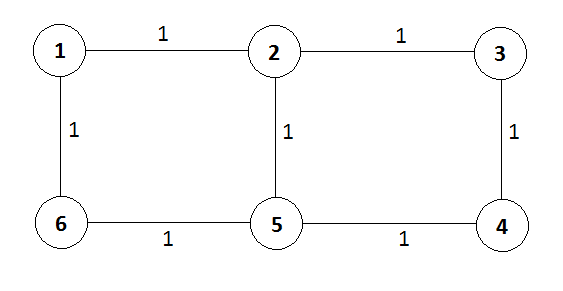
\includegraphics{G:/Genetico/LIBRO_TESIS/04.ListaFiguras/6nodos}
\par\end{centering}
\caption{6 node network topology.}
\label{topology_6nodes_figure}
\end{figure}

\begin{figure}
\begin{centering}
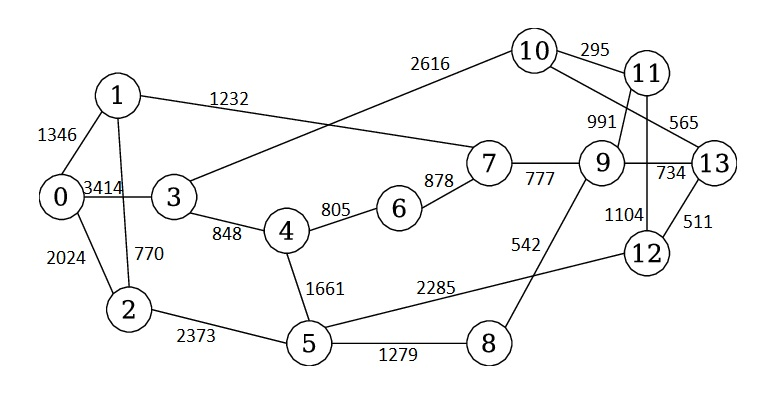
\includegraphics[scale=0.6]{G:/Genetico/LIBRO_TESIS/04.ListaFiguras/nsf_topology}
\par\end{centering}
\caption{Topology of NSF network of 14 nodes with distance in kilometers}
\label{topology_nsf_figure}
\end{figure}

\begin{figure}
\begin{centering}
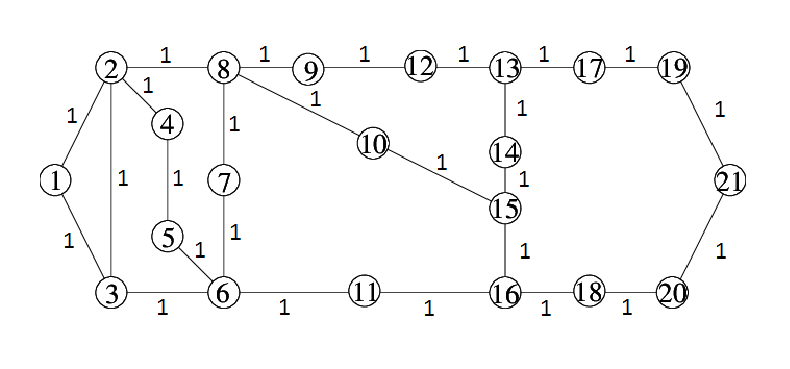
\includegraphics{G:/Genetico/LIBRO_TESIS/04.ListaFiguras/arpa-2}
\par\end{centering}
\caption{21-node Arpa-2 network topology}
\label{topology_arpa-2_figure}
\end{figure}

The traffic loads used were of the all-to-all type, that is, each
node of the network makes a transfer request to all other nodes in
the network. In addition, said traffic loads were divided into two
types: uniform traffic load and random traffic load. In the first,
all the demands request the same amount of FS, the requested quantities
were: 50, 100, 150 and 200 FS. For the random loads, they were also
divided into 4 categories but these quantities were used as the maximum
quantity, that is, for the category of 50 FS, for each demand a random
value between 1 and 50 was generated as requested amount of FS; for
the category of 100, for each demand a random value between 1 and
100 was generated as requested quantity of FS; for the category of
150, for each demand a random value between 1 and 150 was generated
as requested quantity of FS; and finally for the category of 200 for
each demand, a random value between 1 and 200 was generated as requested
quantity of FS.

Another variant that was taken into account for the execution of the
tests was the quantity of precalculated shorter routes, that is, the
value of k. The executions of the MOGA and the GA were made with the
following values of k = 1, 2, 3, 4, 5, 6 and 7, except for the topology
of 6 nodes since in this topology there are up to 3 paths for each
pair of nodes The MOILP was executed with the following values of
k: for the topology of 6 nodes, k = 1, 2 and 3 were used with a time
limit of 2 hours; for the NSF topology a time limit of 4 hours was
defined and results were obtained with k = 1, 2, 3, 4 and 5, except
for the demand scenarios of 200 FS in which only results were obtained
up to k = 4; and for the ARPA-2 topology, a time limit of 4 hours
was also defined and results were obtained only for k = 1. The limitation
in the executions of the MOILP is given by the size of the topologies,
since the ILP implementations are not Generally scalable.

For the executions of the MOGA, the values shown in Table \ref{tabla:moga_params}
were used as evolutionary parameters.

Since the MOGA and the GA are stochastic algorithms, each execution
can present different results. Taking into account this factor, with
the MOGA several executions were carried out for each proposed scenario.
The number of executions per scenario is defined by the parameter
Quantity of independent runs in Table \ref{tabla:moga_params}.

The final results of the MOGA are the average values obtained from
all the executions of each scenario, that is, from 30 independent
runs performed for a scenario, the values of the objective functions
were averaged and said values are those presented in the results.

 \begin{table}[!t] 	
	\centering 	
		\caption{Parameters used for the execution of the MOGA.} 	
		\begin{tabular}{*{2}{|c}|} 		
			\hline 		
			\scriptsize {\textbf{Parameter}} & \scriptsize {\textbf{Value}} \\ 		
			\hline 		
			\scriptsize {Size of the population} & \scriptsize {100} \\ 		
			\hline 		
			\scriptsize {Probability of mutation} & \scriptsize {2\%} \\ 		
			\hline 		
			\scriptsize {Stop criterion} & \scriptsize {5 minutos de ejecuci�n} \\ 		
			\hline 		
			\scriptsize {Number of independent runs} & \scriptsize {30} \\ 		
			\hline 	
		\end{tabular} 	
		\label{tabla:moga_params} 
\end{table} 

\begin{table}[!t] 	
	\centering 	
	\caption{Scenarios of executions.} 	
	\begin{tabular}{ | c | c | >{\centering}m{4,7cm} | c |} 		
		\hline 		
		\scriptsize {\textbf{Topology}} & 
		\scriptsize {\textbf{K}}  & 
		\scriptsize {\textbf{Load}}  & 
		\scriptsize {\textbf{Time}}\\ 		
		\hline 		
		\scriptsize {6-nodes} & \scriptsize {1, 2, 3} & 
		\scriptsize{Uniform 50, 100, 150, 200 Aleatoria: 1-50, 1-100, 1-150, 1-200} & 
		\scriptsize{MOILP: 2 hs, MOGA: 5$\cdot$30 = 150 minutes} \\ 		
		\hline 		
		\scriptsize {NSF} & \scriptsize {1, 2, 3, 4, 5, 6} & 
		\scriptsize{Uniform 50, 100, 150, 200 Aleatoria: 1-50, 1-100, 1-150, 1-200} & 
		\scriptsize{MOILP: 4 hs, MOGA: 5$\cdot$30 = 150 minutes} \\ 		
		\hline 		
		\scriptsize {ARPA-2} & \scriptsize {1, 2, 3, 4, 5, 6} & 
		\scriptsize{Uniform 50, 100, 150, 200 Aleatoria: 1-50, 1-100, 1-150, 1-200} & 
		\scriptsize{MOILP: 4 hs, MOGA: 5$\cdot$30 = 150 minutes} \\ 		
		\hline 	
	\end{tabular} 	
	\label{tabla:escenarios} 
\end{table} 

In Table \ref{tabla:escenarios}, we can see a summary of the executed
scenarios. The topologies used are shown, the values of K for each
topology, the traffic loads (which were divided into uniform load
and random load), and the execution time which, in the case of MOILP,
represent the time limit of defined execution, and in the case of
the MOGA, they represent the total execution time, since for each
independent execution 5 minutes were defined as stopping criteria
and 30 scenarios were performed for each scenario.

Basically, given a scenario consisting of a topology, a number of
routes and traffic load, we proceed to:

\begin{enumerate}     
	\item Calculate a MOILP solution 
	\item Calculate 30 MOGA solutions 
	\item Calculate average values of the 30 MOGA solutions of the objective and Fitness functions 
	\item Calculate 30 GA solutions 
	\item Calculate average values of the 30 GA solutions of the objective functions and Fitness 
	\item Perform analysis of the solutions
\end{enumerate} 

Based on these steps, the following experimental results are presented.

\subsection{Uniform Load Results: MOILP vs MOGA}

In this section we analyze all the results of the objective and fitness
functions, MOILP and MOGA. 

The Figures \ref{6nodos_ilp_fitness}, \ref{6nodos_ilp_fs}, \ref{6nodos_ilp_distance}
and \ref{6nodos_ilp_cost} show the values obtained by the Fitness
MOILP, maximum FS, total distance and total cost, repectively, for
the topology of 6 nodes. The value shown in the vertical axis is the
value of the objective function, and results were obtained up to k
= 3, since with a topology of 6 nodes there are no more than 3 possible
paths for each pair of nodes. When analyzing the Figure \ref{6nodos_ilp_fitness}
it can be seen that having 2 possible ways the fitness value improves,
that is, with k = 2 a great improvement was obtained compared to k
= 1.

It can be observed that by having two possible routes to satisfy the
demands, a second route was used in one or several demands, which
increased the value of the total distance traveled as shown in Figure
\ref{6nodos_ilp_distance}, since the first route is the shortest.
But using a longer route produced a better use of the available spectrum,
since for k = 2, in Figure \ref{6nodos_ilp_fs} a decrease in the
maximum FS used is observed.

Another observation that can be made about these results is that the
greatest improvement was obtained from k = 1 to k = 2, since with
k = 3 practically the fitness value is maintained.

With the results mentioned above, the proposed MOILP implementation
is validated. The same behavior is observed for the topology NSF-14
in the Figures \ref{nsf-14_ilp_fitness}, \ref{nsf-14_ilp_fs}, \ref{nsf-14_ilp_distance}
and \ref{nsf-14_ilp_cost} obtaining results up to k = 5 except for
the 200 FS load that could only be calculated with solutions up to
k = 4. For the ARPA-2 topology, only solutions with k = 1 could be
calculated.

The Figures \ref{6nodos_moga1_fitness}, \ref{6nodos_moga1_fs}, \ref{6nodos_moga1_distance}
and \ref{6nodos_moga1_cost} show the values of fitness, maximum FS,
total distance, and total cost, respectively, obtained by the MOGA
for the topology of 6 nodes. It can be observed that it manages to
obtain practically the same results as the MOILP with values close
to the optimum.

The results obtained by the MOGA for the fitness and the objective
functions of the topology NSF-14, are shown in the Figures \ref{nsf-14_moga1_fitness},
\ref{nsf-14_moga1_fs}, \ref{nsf-14_moga1_distance} and \ref{nsf-14_moga1_cost}.
It can also be observed that the most significant improvement occurs
with k = 2, from k = 3 almost no changes are seen in the results and
it is converging.

Finally, the Figures \ref{arpa-2_ilp_fitness}, \ref{arpa-2_moga1_fs},
\ref{arpa-2_moga1_distance} y \ref{arpa-2_moga1_cost} show the values
of fitness and objective functions for the ARPA-2 topology obtained
by the MOGA. When observing the fitness values obtained by both implementations,
it can be verified that for all values of k in the 3 topologies, the
MOILP surpassed the results obtained by the MOGA, however, the MOGA
presents results very close to the optimum generating promising solutions.

\begin{figure}
\begin{centering}
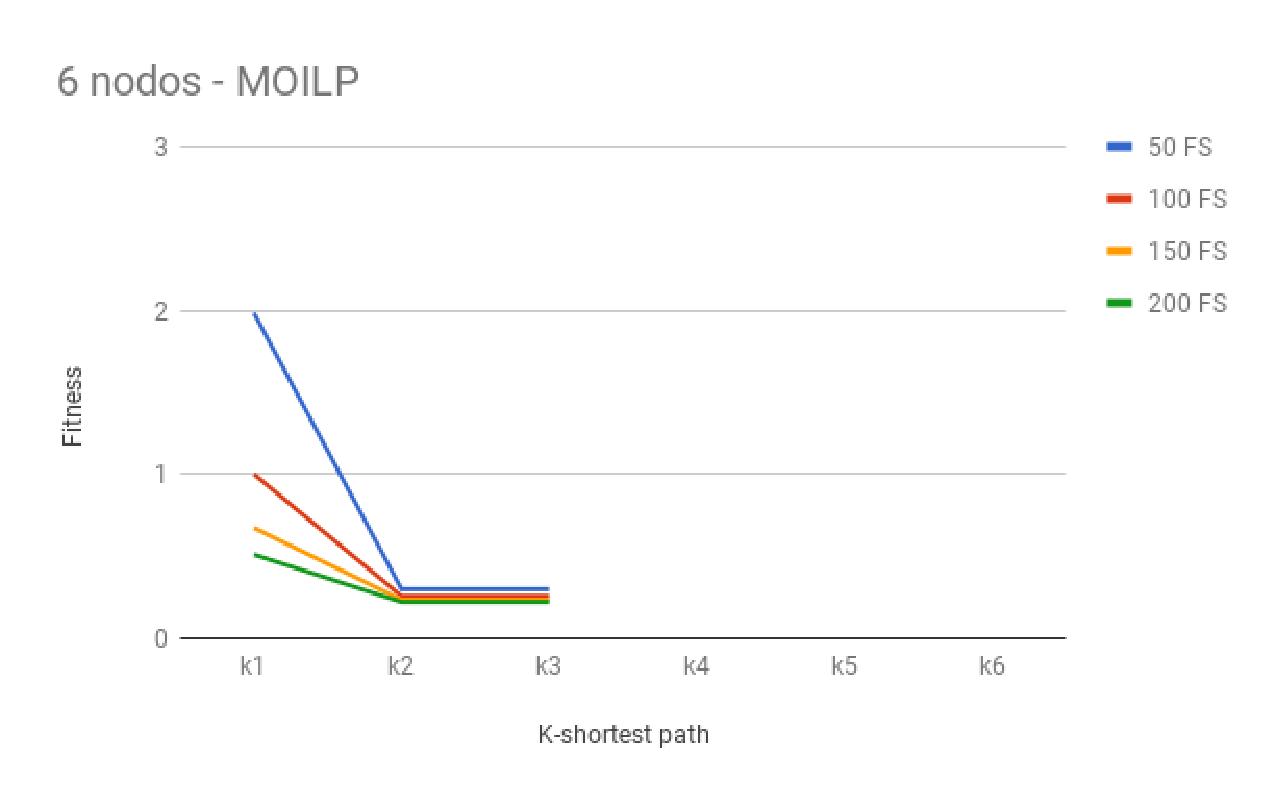
\includegraphics[scale=0.6]{G:/Genetico/LIBRO_TESIS/resulYsapy/resultados/6nodos_uniforme_ilp_fitness}
\par\end{centering}
\caption{Fitness obtained by MOILP for topology 6 nodes with uniform load.}
\label{6nodos_ilp_fitness}
\end{figure}

\begin{figure}
\begin{centering}
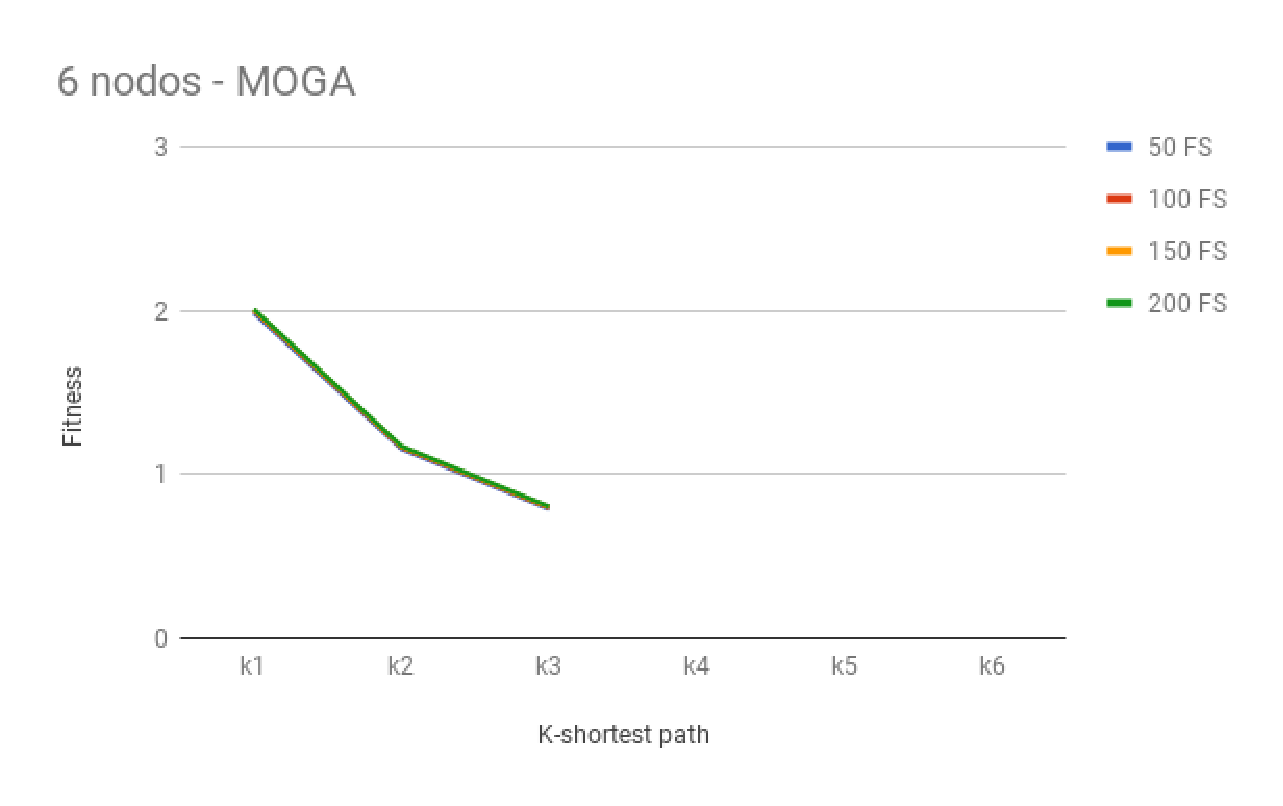
\includegraphics[scale=0.6]{G:/Genetico/LIBRO_TESIS/resulYsapy/resultados/6nodos_uniforme_moga1_fitness}
\par\end{centering}
\caption{Average fitness obtained by the MOGA talks topology of 6 nodes with
uniform charge}
\label{6nodos_moga1_fitness}
\end{figure}

\begin{figure}
\begin{centering}
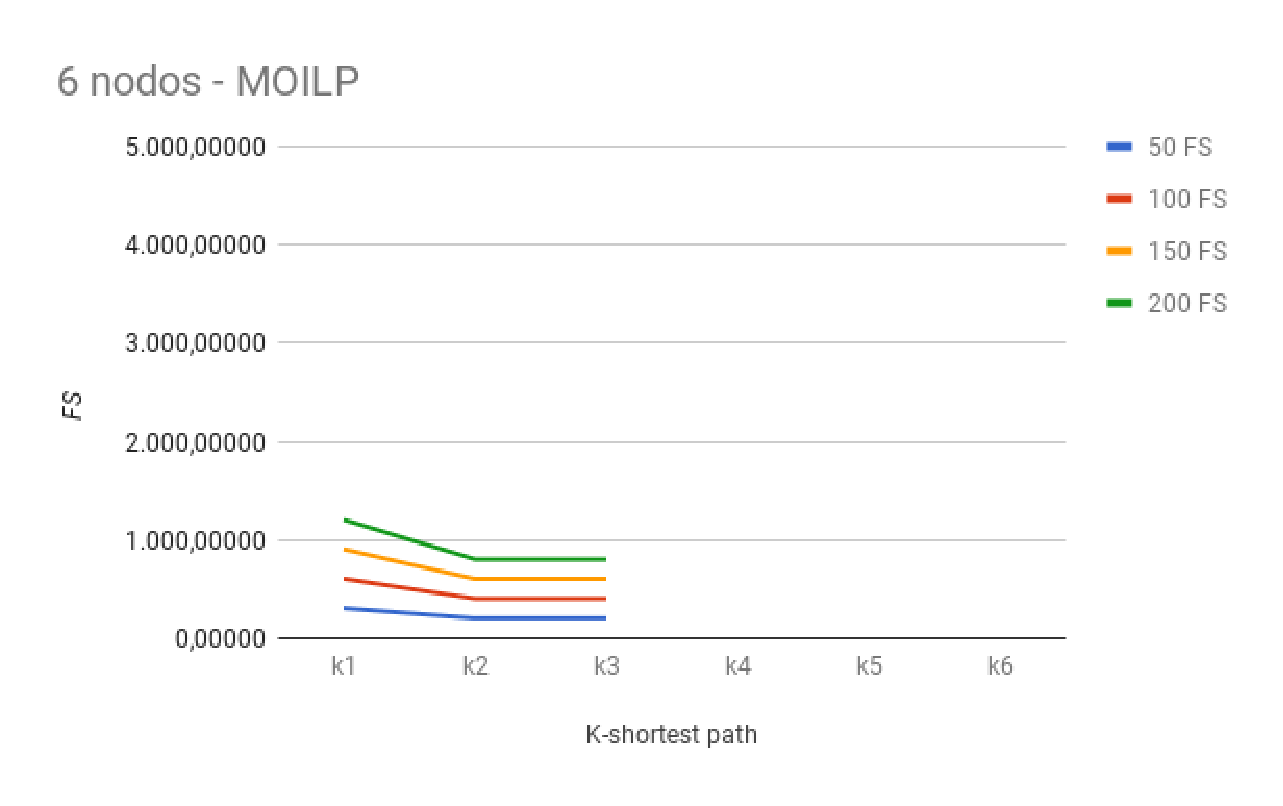
\includegraphics[scale=0.6]{G:/Genetico/LIBRO_TESIS/resulYsapy/resunif/6nodos_uniforme_ilp_fs}
\par\end{centering}
\caption{Maximum FS obtained by the MOILP for the topology of 6 nodes with
uniform load.}
\label{6nodos_ilp_fs}
\end{figure}

\begin{figure}
\begin{centering}
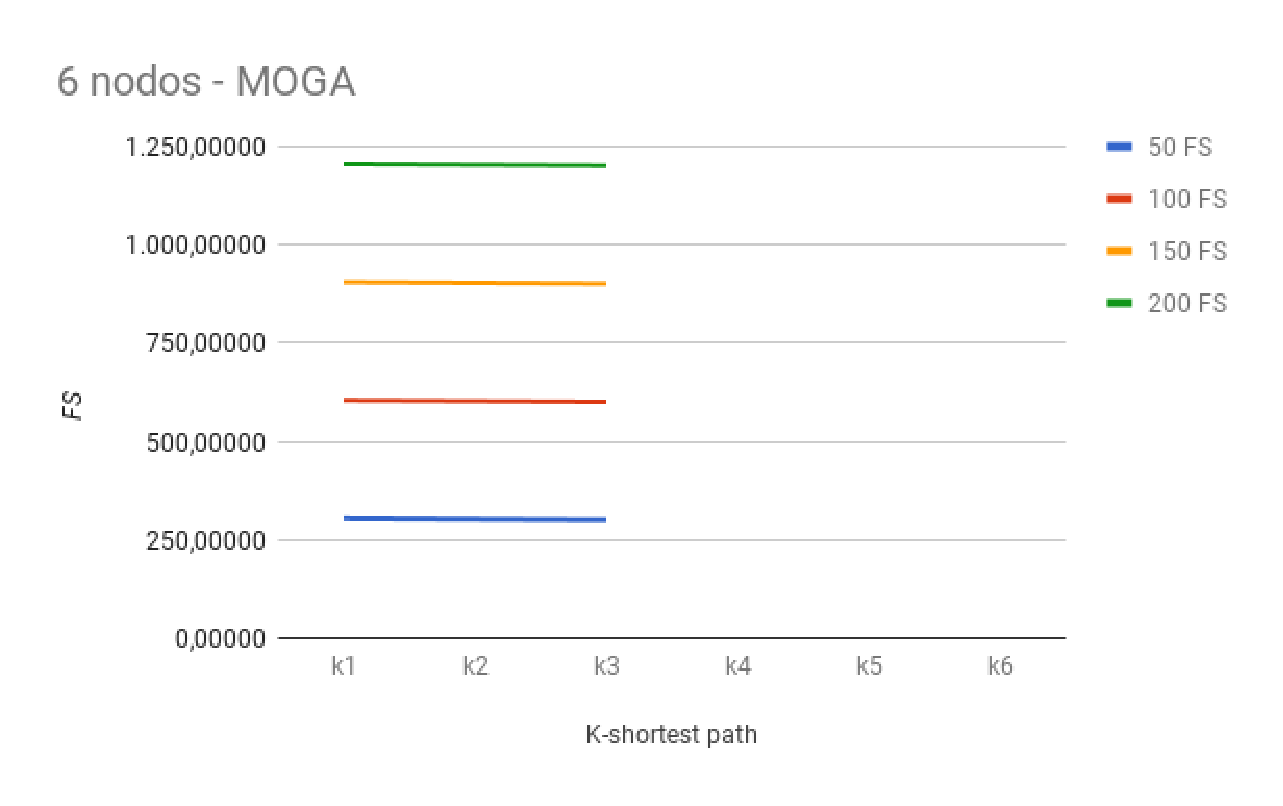
\includegraphics[scale=0.6]{G:/Genetico/LIBRO_TESIS/resulYsapy/resunif/6nodos_uniforme_moga1_fs}
\par\end{centering}
\caption{Maximum average FS obtained by the MOGA for the topology of 6 nodes
with uniform load.}
\label{6nodos_moga1_fs}
\end{figure}

\begin{figure}
\begin{centering}
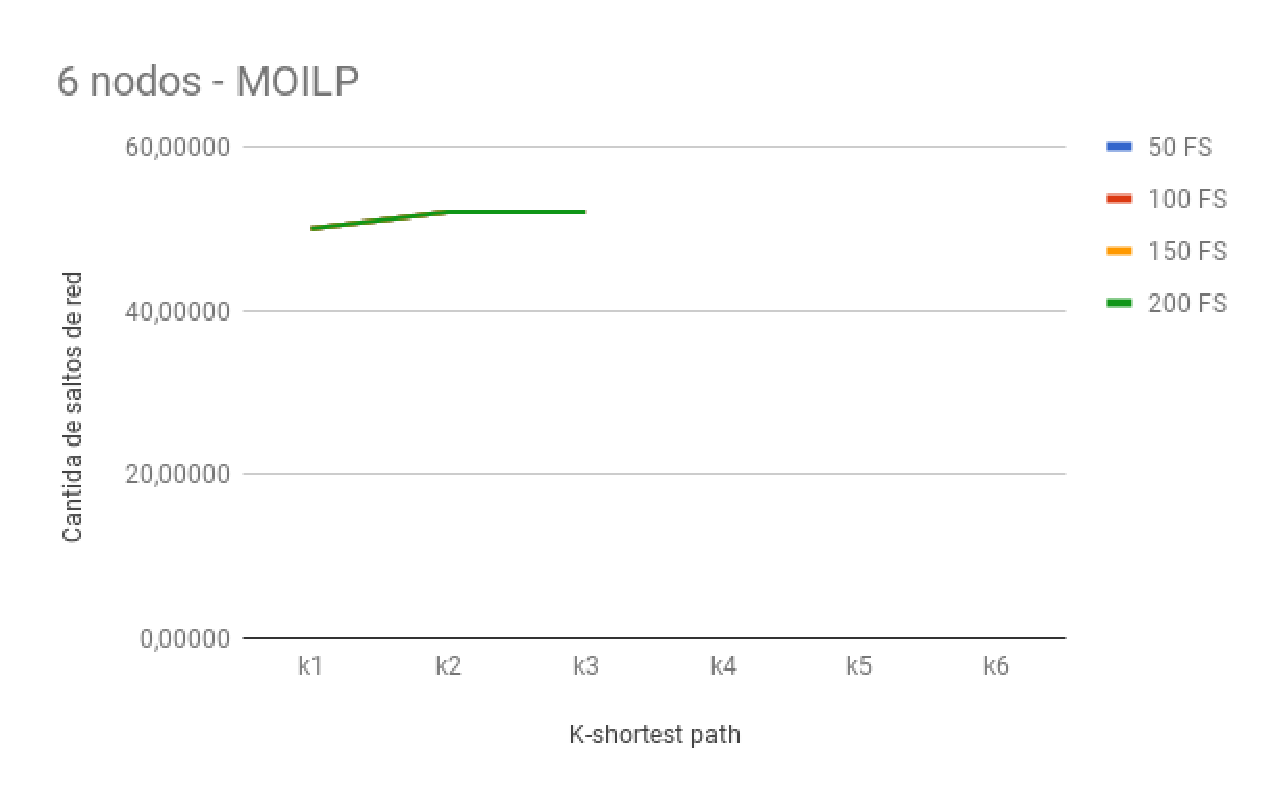
\includegraphics[scale=0.6]{G:/Genetico/LIBRO_TESIS/resulYsapy/resunif/6nodos_uniforme_ilp_distancia}
\par\end{centering}
\caption{Total distance obtained by the MOILP for the topology of 6 nodes with
uniform load.}
\label{6nodos_ilp_distance}
\end{figure}

\begin{figure}
\begin{centering}
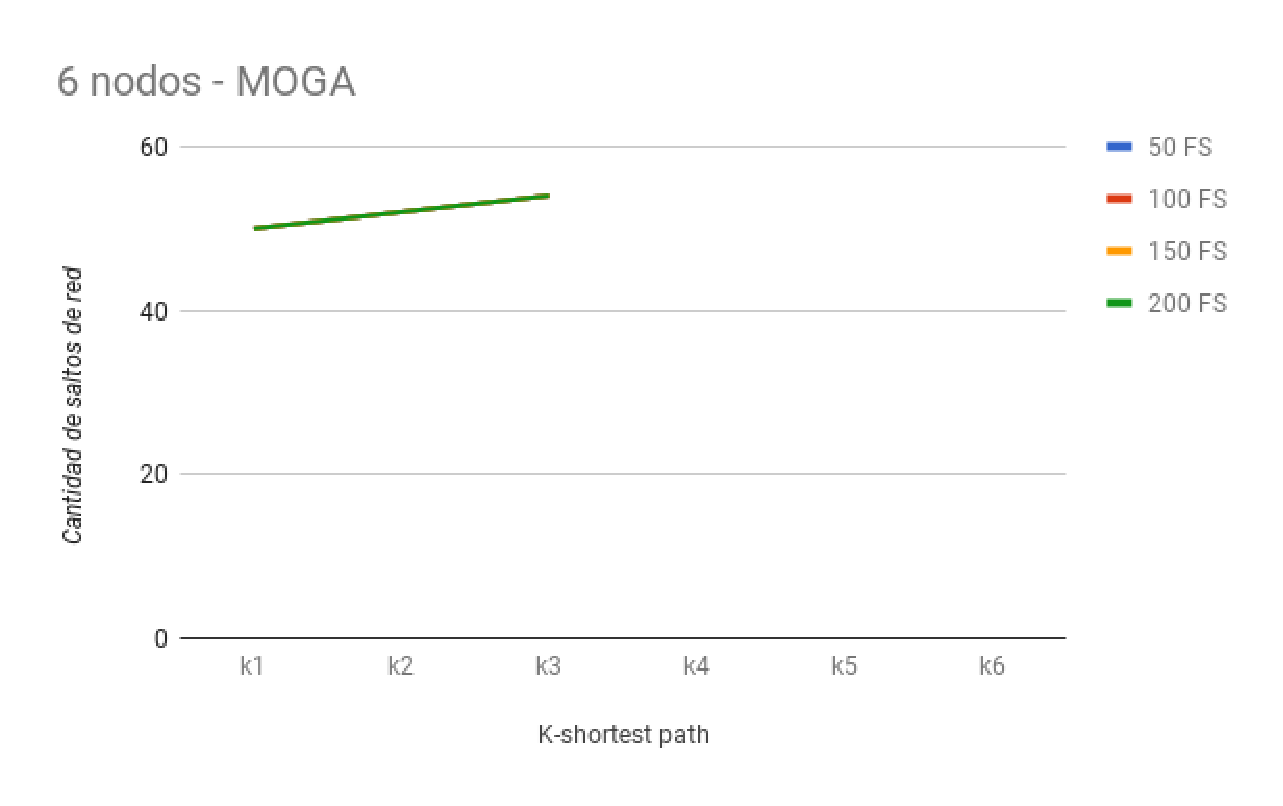
\includegraphics[scale=0.6]{G:/Genetico/LIBRO_TESIS/resulYsapy/resunif/6nodos_uniforme_moga1_distancia}
\par\end{centering}
\caption{Average total distance obtained by the MOGA for the topology of 6
nodes with uniform load}
\label{6nodos_moga1_distance}
\end{figure}

\begin{figure}
\begin{centering}
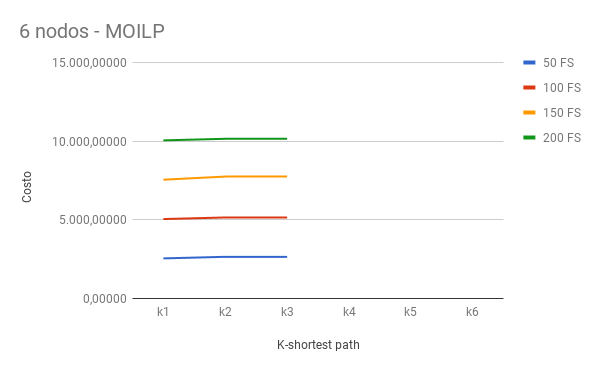
\includegraphics[scale=0.6]{G:/Genetico/LIBRO_TESIS/resulYsapy/resunif/6nodos_uniforme_ilp_costo}
\par\end{centering}
\caption{Total cost obtained by MOILP for the topology of 6 nodes with uniform
load.}
\label{6nodos_ilp_cost}
\end{figure}

\begin{figure}
\begin{centering}
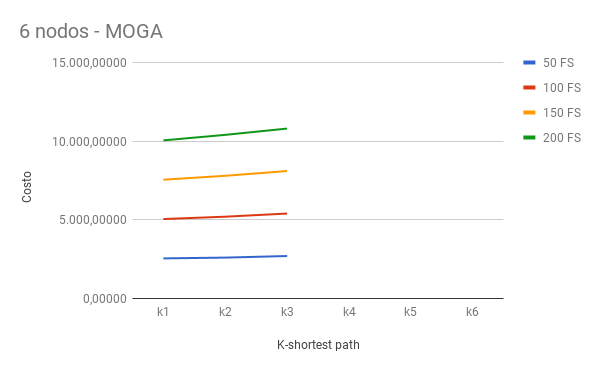
\includegraphics[scale=0.6]{G:/Genetico/LIBRO_TESIS/resulYsapy/resunif/6nodos_uniforme_moga1_costo}
\par\end{centering}
\caption{Average total cost obtained by the MOGA for the topology 6 nodes with
uniform load.}
\label{6nodos_moga1_cost}
\end{figure}

\begin{figure}
\begin{centering}
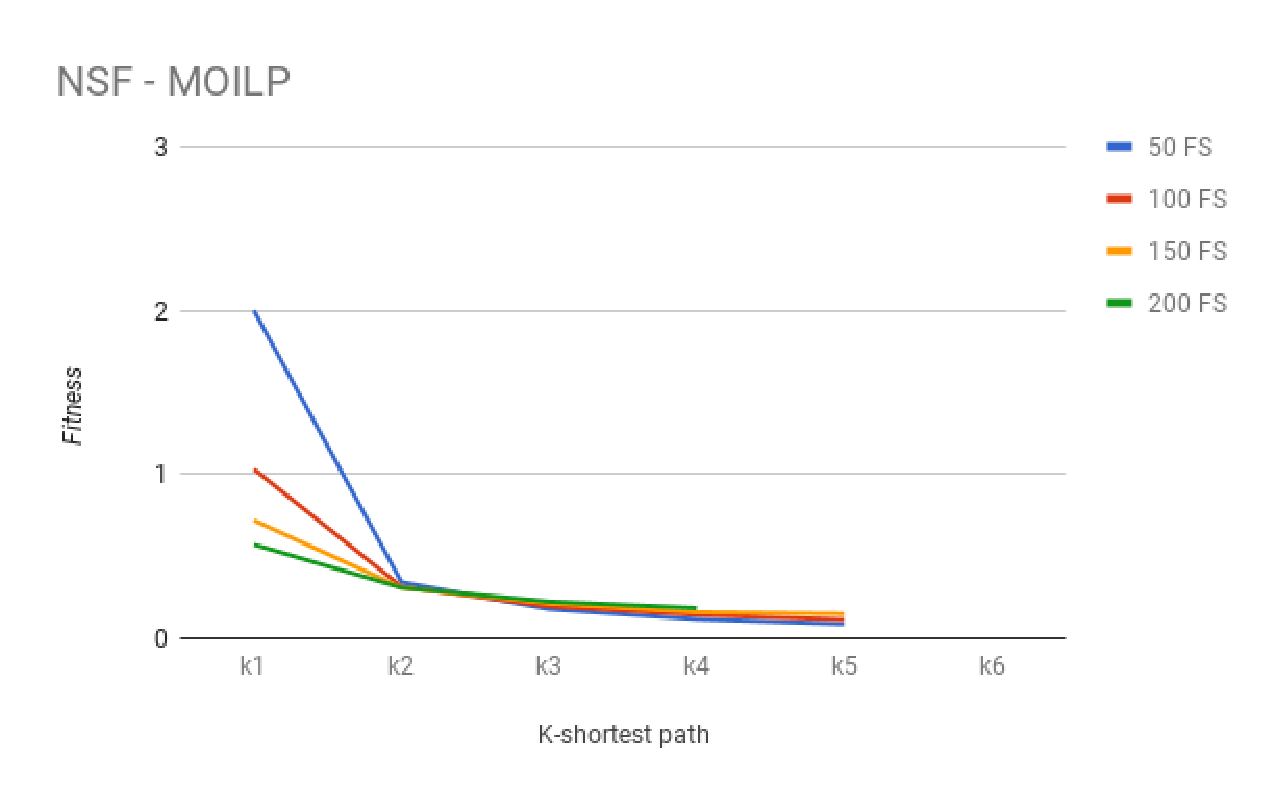
\includegraphics[scale=0.6]{G:/Genetico/LIBRO_TESIS/resulYsapy/resultados/nsf_uniforme_ilp_fitness}
\par\end{centering}
\caption{Fitness obtained by MOILP for topology NSF-14 with uniform load.}
\label{nsf-14_ilp_fitness}
\end{figure}

\begin{figure}
\begin{centering}
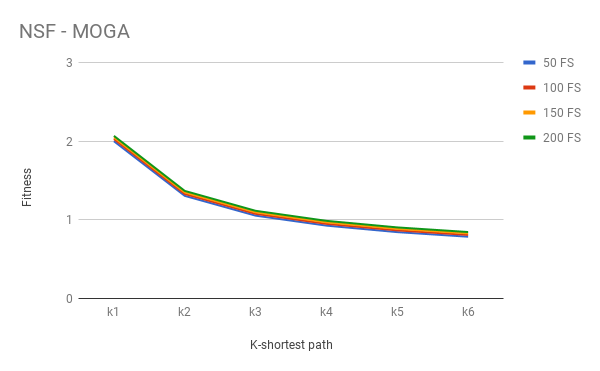
\includegraphics[scale=0.6]{G:/Genetico/LIBRO_TESIS/resulYsapy/resultados/nsf_uniforme_moga1_fitness}
\par\end{centering}
\caption{Average fitness obtained by the MOGA talks topology of NSF-14 with
uniform charge}
\label{nsf-14_moga1_fitness}
\end{figure}

\begin{figure}
\begin{centering}
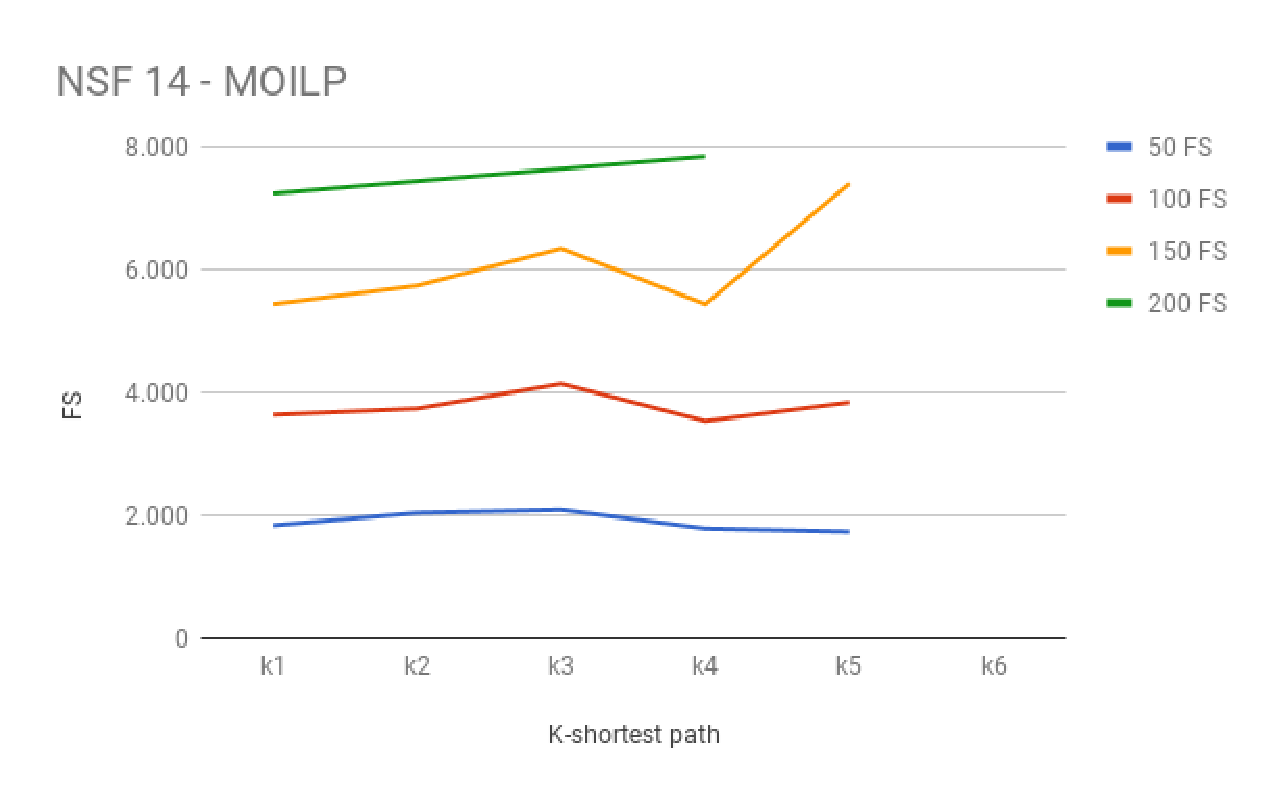
\includegraphics[scale=0.6]{G:/Genetico/LIBRO_TESIS/resulYsapy/resunif/nsf_uniforme_ilp_fs}
\par\end{centering}
\caption{Maximum FS obtained by the MOILP for the topology of NSF-14 with uniform
load.}
\label{nsf-14_ilp_fs}
\end{figure}

\begin{figure}
\begin{centering}
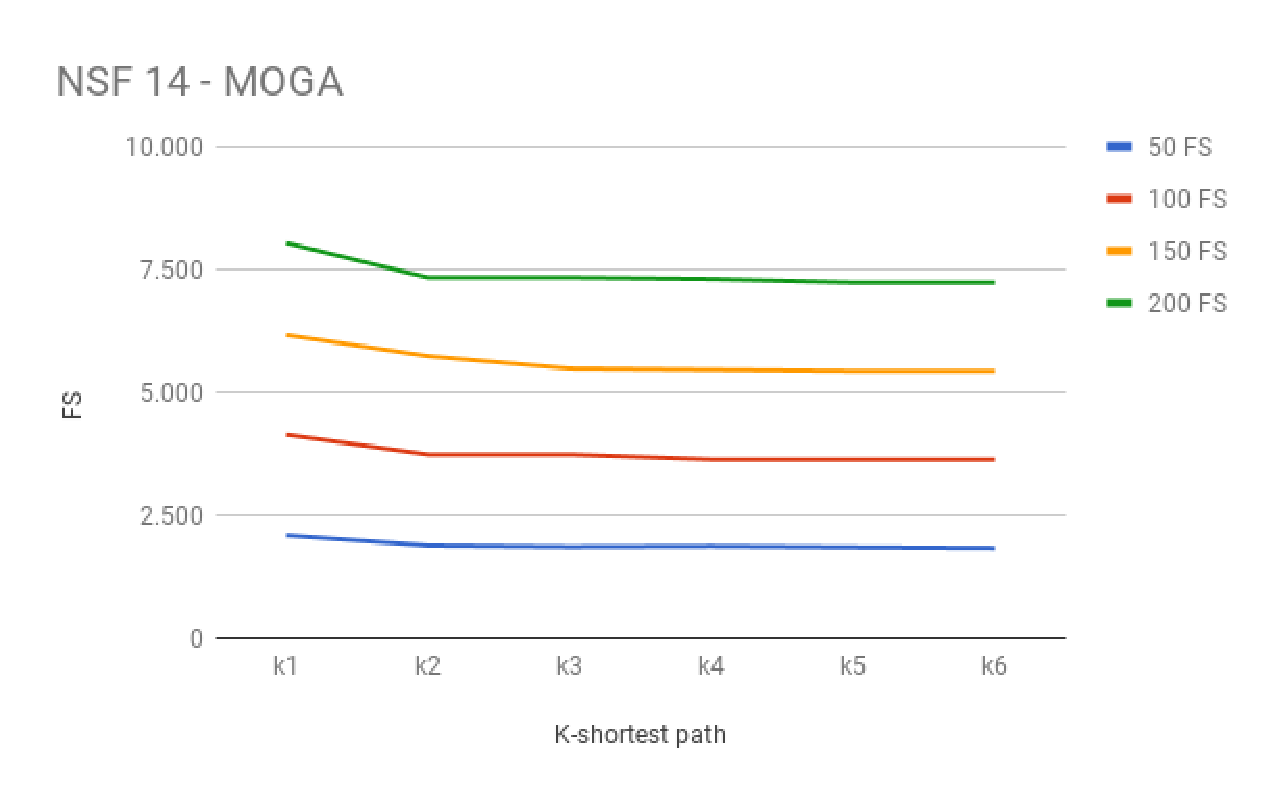
\includegraphics[scale=0.6]{G:/Genetico/LIBRO_TESIS/resulYsapy/resunif/nsf_uniforme_moga1_fs}
\par\end{centering}
\caption{Maximum average FS obtained by the MOGA for the topology of NSF-14
with uniform load.}
\label{nsf-14_moga1_fs}
\end{figure}

\begin{figure}
\begin{centering}
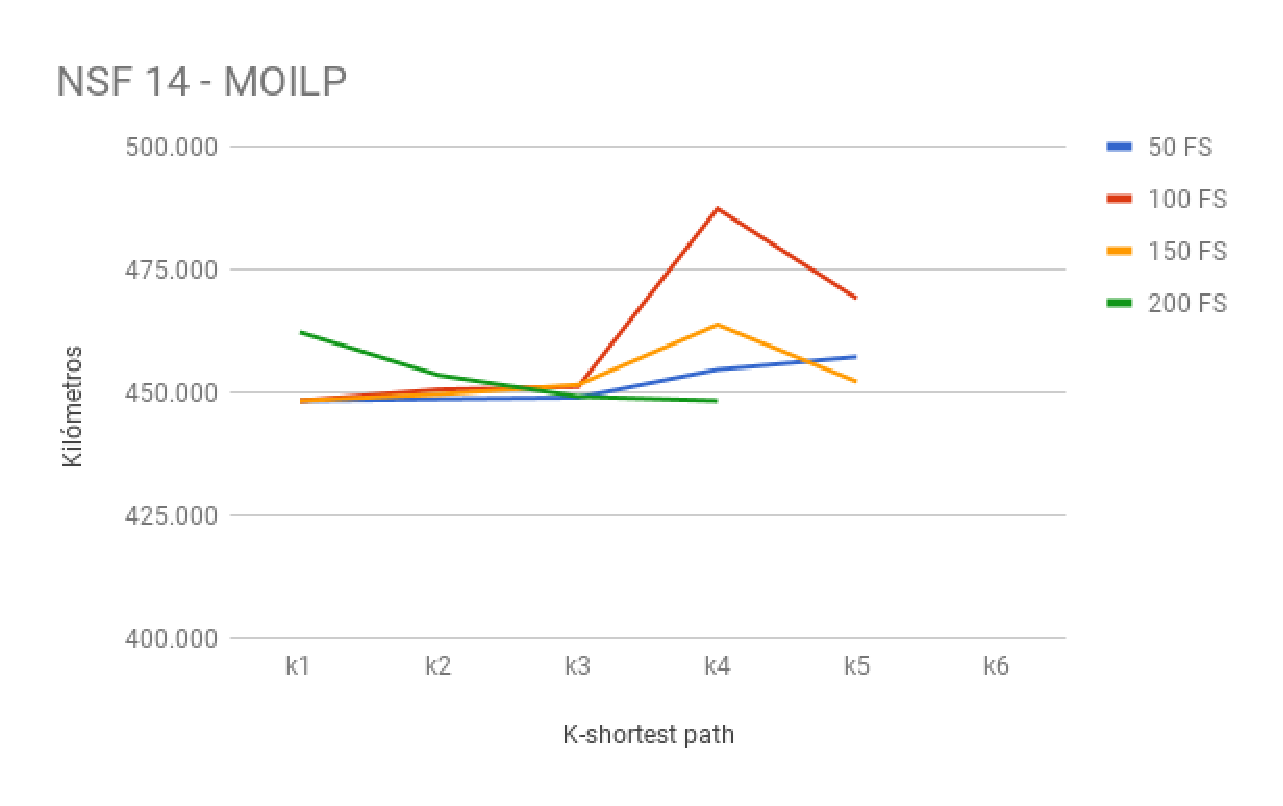
\includegraphics[scale=0.6]{G:/Genetico/LIBRO_TESIS/resulYsapy/resunif/nsf_uniforme_ilp_distancia}
\par\end{centering}
\caption{Total distance obtained by the MOILP for the topology of NSF-14 with
uniform load.}
\label{nsf-14_ilp_distance}
\end{figure}

\begin{figure}
\begin{centering}
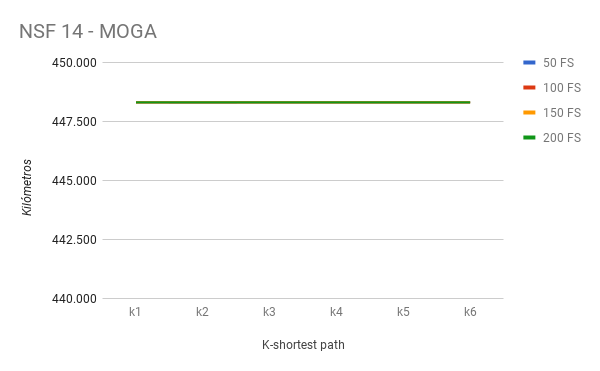
\includegraphics[scale=0.6]{G:/Genetico/LIBRO_TESIS/resulYsapy/resunif/nsf_uniforme_moga1_distancia}
\par\end{centering}
\caption{Average total distance obtained by the MOGA for the topology of NSF-14
with uniform load}
\label{nsf-14_moga1_distance}
\end{figure}

\begin{figure}
\begin{centering}
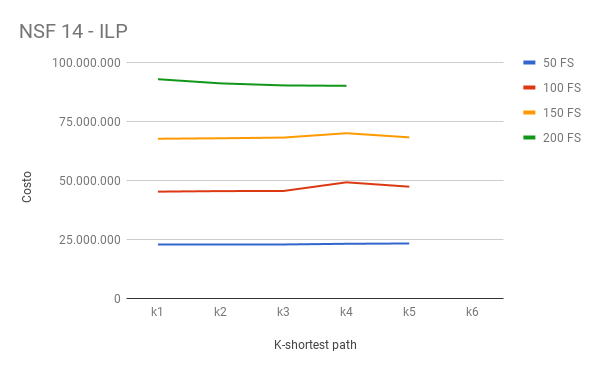
\includegraphics[scale=0.6]{G:/Genetico/LIBRO_TESIS/resulYsapy/resunif/nsf_uniforme_ilp_costo}
\par\end{centering}
\caption{Total cost obtained by MOILP for the topology of NSF-14 with uniform
load.}
\label{nsf-14_ilp_cost}
\end{figure}

\begin{figure}
\begin{centering}
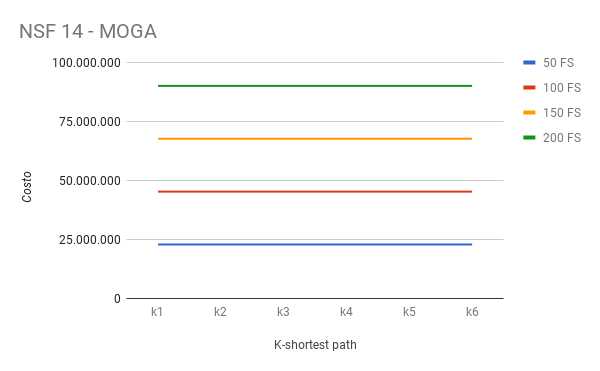
\includegraphics[scale=0.6]{G:/Genetico/LIBRO_TESIS/resulYsapy/resunif/nsf_uniforme_moga1_costo}
\par\end{centering}
\caption{Average total cost obtained by the MOGA for the topology NSF-14 with
uniform load.}
\label{nsf-14_moga1_cost}
\end{figure}

\begin{figure}
\begin{centering}
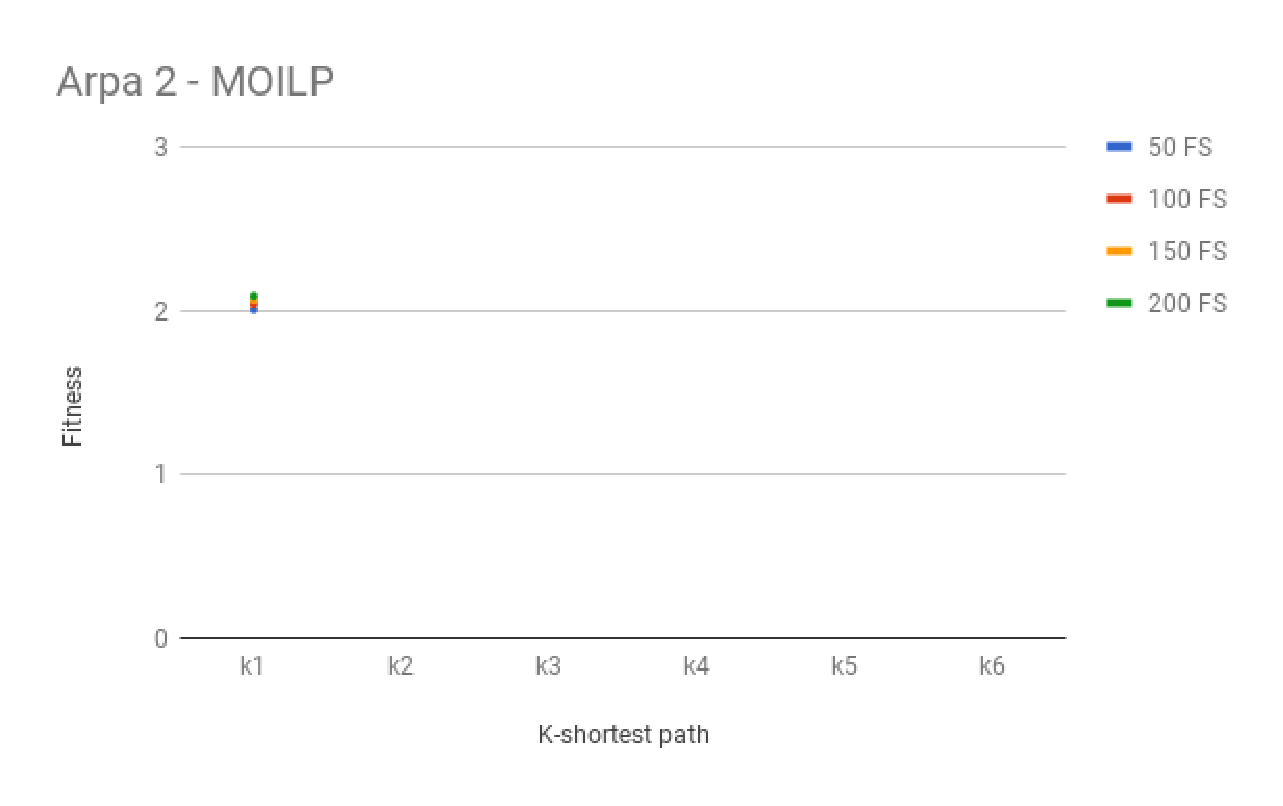
\includegraphics[scale=0.6]{G:/Genetico/LIBRO_TESIS/resulYsapy/resultados/arpa_uniforme_ilp_fitness}
\par\end{centering}
\caption{Fitness obtained by MOILP for topology ARPA-2 with uniform load.}
\label{arpa-2_ilp_fitness}
\end{figure}

\begin{figure}
\begin{centering}
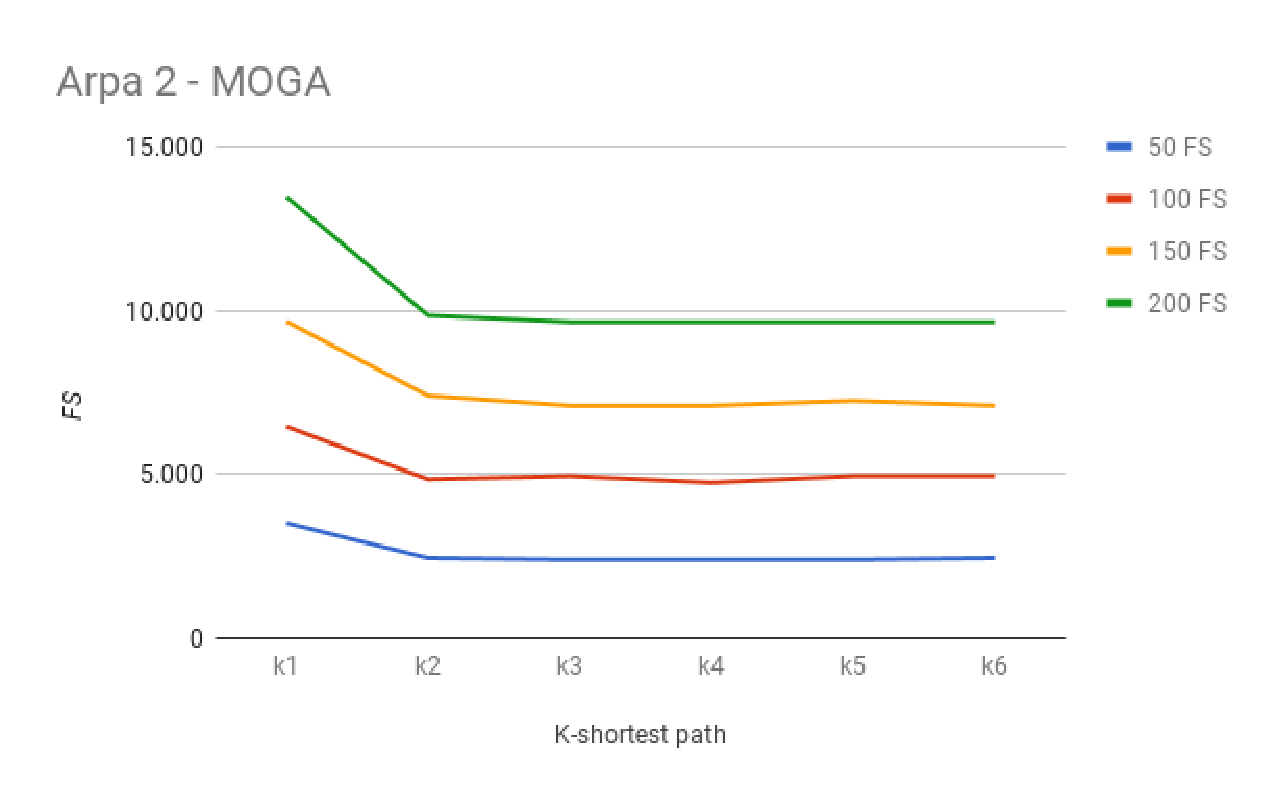
\includegraphics[scale=0.6]{G:/Genetico/LIBRO_TESIS/resulYsapy/resunif/arpa_uniforme_moga1_fs}
\par\end{centering}
\caption{Maximum average FS obtained by the MOGA talks topology of ARPA-2 with
uniform charge}
\label{arpa-2_moga1_fs}
\end{figure}

\begin{figure}
\begin{centering}
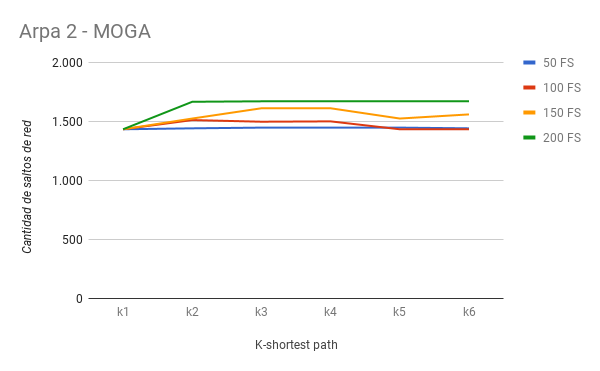
\includegraphics[scale=0.6]{G:/Genetico/LIBRO_TESIS/resulYsapy/resunif/arpa_uniforme_moga1_distancia}
\par\end{centering}
\caption{Total distance obtained by the MOGA for the topology of ARPA-2 with
uniform load.}
\label{arpa-2_moga1_distance}
\end{figure}

\begin{figure}
\begin{centering}
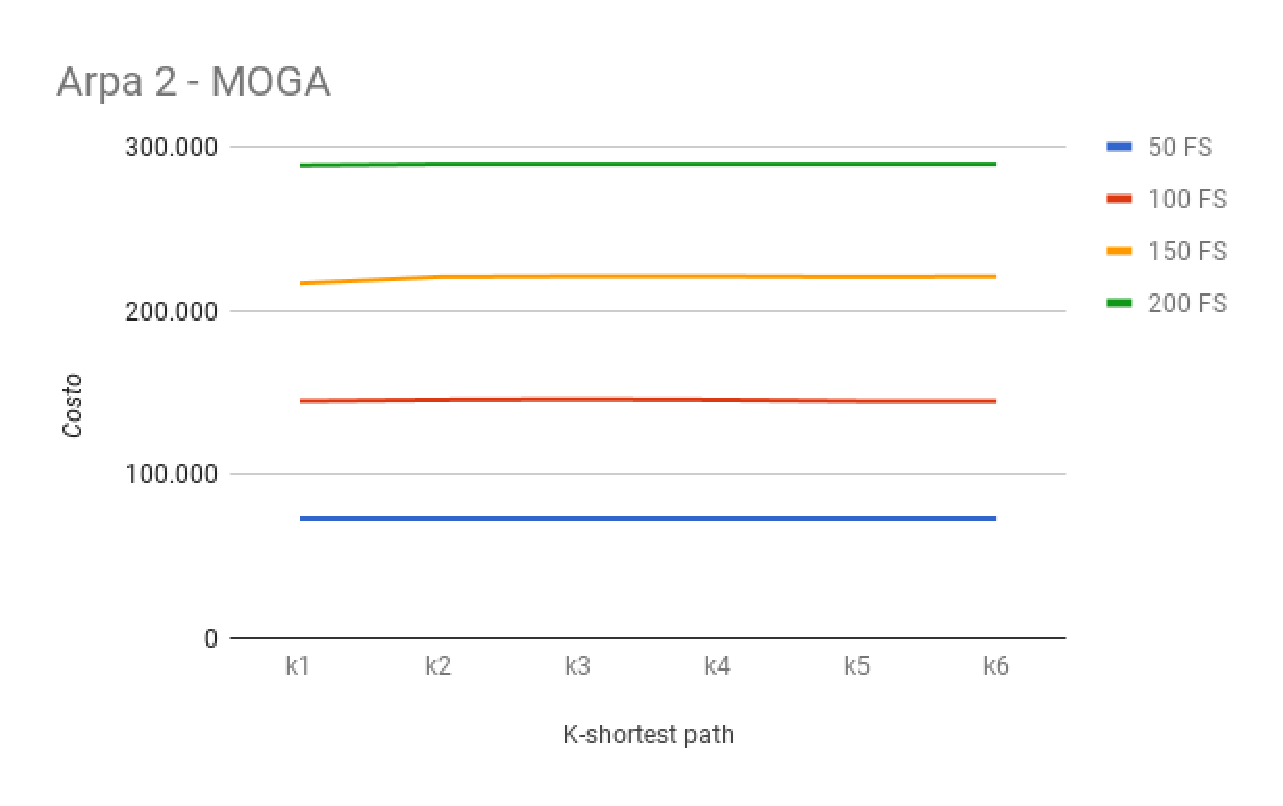
\includegraphics[scale=0.6]{G:/Genetico/LIBRO_TESIS/resulYsapy/resunif/arpa_uniforme_moga1_costo}
\par\end{centering}
\caption{Average total cost obtained by the MOGA for the topology of ARPA-2
with uniform load.}
\label{arpa-2_moga1_cost}
\end{figure}


\section{NSGAII{*} vs NSGS II}

In this section we present the difference with the work proposed in
\cite{moga-rsa-dao} and the work presented by us, in addition the
results of the experimental tests are presented and analyzed. The
work proposed in \cite{moga-rsa-dao}, presents the multi-objective
RSA problem and its associated algorithm model. Each request has many
possible routes, and in each routing it has several spectrum assignment
options. The problem is to minimize the spectrum width to support
all requests and minimize the overall cost of the spectrum in the
link. 

The objective function for the work proposed in \cite{moga-rsa-dao}
is as follows: there are two objectives associated with each chromosome.
The first objective $f_{1}$, is the width of the spectrum that indicates
the maximum indexed slice used in the network. The second objective
$f_{2}$ is the total cost of the spectrum link. Given a chromosome,
the route and channel are calculated for each demand. After attending
each demand sequentially and without any sort of ordering, the spectrum
availabilities vector of each link is updated. 

In this developed work, which is an extension of the work presented
in \cite{engopt} which has an approach based on weighted sum, a pure
multi-objective approach with Pareto fronts is presented. In our work,
as in \cite{moga-rsa-dao} it has many possible routes, and in each
routing it has several spectrum assignment options. The problem is
to minimize the spectrum width to support all requests and minimize
the overall cost of the link spectrum. The same objective function
is taken from \cite{moga-rsa-dao} and the requests are handled as
follows: applications are ordered from highest to lowest, defined
by the highest possible cost of said request, the first 30\% of said
list is attended in the first place, while the remaining 70\% is treated
in a random manner, unlike \cite{moga-rsa-dao} it is a random ordering. 

The tests carried out considering different types of traffic load,
on the NSF topology (Figure \ref{topology_nsf_figure}), different
K values (paths) and different amounts of demands, try to replicate
various possible scenarios of the problem to solve. The experimental
tests carried out show that our proposal for the ordering of the requests
presents promising results. 

\subsection{Testing environment }

The experiments were performed on a computer with an Intel Core i3
processor (3.40 GHz) and 8 GB of RAM. The implementation and execution
of the MOEAs were carried out with JAVA 8. 

The traffic loads used were of the all-to-all type, that is, each
node of the network makes a transfer request to all others in the
network. In addition, the type of traffic load was random. The loads
are divided into 3 categories, 50, 100 and 150 (low, medium, high),
that is to say that for the category of 50 FS, for each demand a random
value between 1 and 50 was generated as a requested quantity of FS;
For category 100, for each demand a random value between 1 and 100
was generated as the requested quantity of FS and for category 150,
a random value of 1 and 150 was generated as requested quantity of
FS. Another variant that was taken into account for the execution
of the tests was the number of shortest routes pre-calculated, that
is, the value K. They were made with the following values of k = 2,
3, 4 and 5 for the network. For the executions of the NSGA II, the
values shown in Table 1 were used as evolutionary parameters. The
metric used for the comparison of the algorithms are hyper-volume
and coverage \cite{engopt}. 

Based on these steps, the experimental results are presented.

\begin{table}
\caption{Parameters used for the execution of the MOEA's}

\centering{}%
\begin{tabular}{cc}
\hline 
\textbf{Parameters} & \textbf{Value}\tabularnewline
\hline 
Size of the population & 50\tabularnewline
\hline 
Probability of mutation & 0.1\tabularnewline
\hline 
Stop Criterion (in minutes) & 5\tabularnewline
\hline 
Number of independent runs & 15\tabularnewline
\hline 
\end{tabular}
\end{table}


\subsection{Hyper-volume Metric }

For the hyper-volume metric you can see the table number 2, for load
type 50 (low), with the number of paths k = 2, our proposed algorithm
of order 30/70 obtains better results before the algorithm without
ordering. For load type 50 (low), with k = 3 paths, again our algorithm
with order 30/70, exceeds the algorithm without ordering. For load
type 50 with k = 4, the algorithm without ordering obtained better
results with our algorithm 30/70. For k = 5 with 50 loading (low),
our algorithm 30/70 obtained good results. For k = 2 with 100 load
(average), the algorithm without ordering obtained better results,
k = 3 with 100 load (average), our algorithm with order 30/70, has
better results before the algorithm without ordering, for k = 4 with
100 load (average), our 30/70 sorting algorithm improves the results
before the algorithm without ordering. For k = 5 with 100 of load
(average), we obtained very good results with respect to the algorithm
without ordination. 

For k = 2 with 150 loading (high), our sort algorithm 30/70 obtained
better results compared to the algorithm without ordering. In k =
3 with 150 loading (high), the algorithm without ordination obtained
good results. Our 30/70 sorting algorithm got better results when
k = 4 with 150 loading (high) compared to the unordered algorithm.
The unordered algorithm had better results when k = 5 and the load
is 150 (high), compared to our 30/70 sorting algorithm.

\subsection{Coverage Metric }

For the coverage metric we analyze the table number 3, where it can
be seen when the load type is 50 (low) and the number of roads k =
2, our ordering algorithm 30/70 obtained a greater coverage before
the algorithm without ordination. For k = 3 with 50 load (low), our
algorithm obtained a greater coverage with respect to the algorithm
without ordering. For when k = 4 and 50 of load (low), the algorithm
without ordination obtained a greater coverage before our algorithm
of ordering 30/70. With k = 5 and the load of 50 (low), our ordering
algorithm 30/70 obtained a better coverage. For load type 100 (average)
with k = 2, the unordered algorithm had better coverage in our ordering
algorithm 30/70. When k = 3 with load type 100 (average), our algorithm
obtained better coverage before the algorithm without ordering. With
a load of 100 (average) and k = 4, our algorithm obtained better coverage
than the algorithm without ordination. When k = 5 and load type 100
(average), our algorithm obtained better coverage than the algorithm
without ordination. 

For load type 150 (high) with k = 2, our algorithm showed better coverage
than the algorithm without ordination, for k = 3 and 150 load (high),
the algorithm without ordination yielded better coverage than our
ordering algorithm. 30/ 70 For k = 4 with 150 loading (high), our
algorithm obtained better coverage before the algorithm without ordering.
For k = 4 with a load of 150 (high), the algorithm without ordering
obtained better coverage. For k = 5 with 150 loading (high), our algorithm
obtained better coverage than the non-ordered algorithm. 
\begin{center}
\begin{table}
\caption{Comparision of algorithms, hyper-volumen metric}

\centering{}%
\begin{tabular}{|>{\raggedright}m{2cm}|>{\centering}m{2cm}|l|l|}
\hline 
\centering{}\textbf{Type of load (low, mid, high)} & \textbf{Number of roads (k)} & \textbf{Sorting Algorithm 30/70} & \textbf{Unsorted Algorithm}\tabularnewline
\hline 
\hline 
\multirow{4}{2cm}{\centering{}50} & 2 & \textbf{0,00450575727952277000} & 0,00373184833987698000\tabularnewline
\cline{2-4} 
 & 3 & \textbf{0,03004763727709010000} & 0,00114619949446014000\tabularnewline
\cline{2-4} 
 & 4 & 0,00107277586229790000 & \textbf{0,00608913898555240000}\tabularnewline
\cline{2-4} 
 & 5 & \textbf{0,01524133420666540000} & 0,01404235292493280000\tabularnewline
\hline 
\multirow{4}{2cm}{\centering{}100} & 2 & 0,00000000040137206552 & \textbf{0,00000000428130203222}\tabularnewline
\cline{2-4} 
 & 3 & \textbf{0,00235590742252450000} & 0,00192187663358532000\tabularnewline
\cline{2-4} 
 & 4 & \textbf{0,00000000625575249301} & 0,00000000039930335062\tabularnewline
\cline{2-4} 
 & 5 & \textbf{0,00000000560063877525} & 0,00000000040004562680\tabularnewline
\hline 
\multirow{4}{2cm}{\centering{}150} & 2 & \textbf{0,00000000437845029918} & 0,00000000027365314370\tabularnewline
\cline{2-4} 
 & 3 & 0,00004759974150804820 & \textbf{0,00063478877339381300}\tabularnewline
\cline{2-4} 
 & 4 & \textbf{0,00036203376622539800} & 0,00003620284610853910\tabularnewline
\cline{2-4} 
 & 5 & 0,00004690367773651360 & \textbf{0,00171967667778795000}\tabularnewline
\hline 
\end{tabular}
\end{table}
\par\end{center}

\begin{center}
\begin{table}
\caption{Comparision of algorithms, coverage metric}

\centering{}%
\begin{tabular}{|>{\centering}m{2cm}|>{\centering}m{2cm}|c|c|}
\hline 
\textbf{Type of load (low, mid, high)} & \textbf{Number of roads (k)} & \textbf{Sorting Algorithm 30/70} & \textbf{Unsorted Algorithm}\tabularnewline
\hline 
\hline 
\multirow{4}{2cm}{\centering{}50} & 2 & \textbf{0,6} & 0,3\tabularnewline
\cline{2-4} 
 & 3 & \textbf{1,0} & 0,0\tabularnewline
\cline{2-4} 
 & 4 & 0,0 & \textbf{1,0}\tabularnewline
\cline{2-4} 
 & 5 & \textbf{0,5} & 0,0\tabularnewline
\hline 
\multirow{4}{2cm}{\centering{}100} & 2 & 0,0 & \textbf{1,0}\tabularnewline
\cline{2-4} 
 & 3 & \textbf{0,3} & 0,0\tabularnewline
\cline{2-4} 
 & 4 & \textbf{1,0} & 0,0\tabularnewline
\cline{2-4} 
 & 5 & \textbf{1,0} & 0,0\tabularnewline
\hline 
\multirow{4}{2cm}{\centering{}150} & 2 & \textbf{1,0} & 0,0\tabularnewline
\cline{2-4} 
 & 3 & 0,0 & \textbf{1,0}\tabularnewline
\cline{2-4} 
 & 4 & \textbf{1,0} & 0,0\tabularnewline
\cline{2-4} 
 & 5 & 0,0 & \textbf{1,0}\tabularnewline
\hline 
\end{tabular}
\end{table}
\par\end{center}



\chapter{CONCLUSIONS AND FUTURE WORK }

According to the exposed results, we can conclude that our algorithm
with ordering obtains better Pareto Fronts, with respect to the algorithm
without ordination. Likewise we conclude that if we give a treatment
to the table of requests, ordering them from highest to lowest, defined
by the highest possible cost of said request, and we divide the table
of requests into two groups, one group of seniors and another group
of random attendance we get better Pareto Fronts. 

As future work to develop we can mention several opportunities: study
the performance of other spectrum assignment algorithms, consider
other strategies of sorting the request to be served, extend this
approaches considering other issues as modulation level assignment
or coded assignment. 


\bibliographystyle{plain}
\bibliography{bibliografia_TESIS_FINAL}

\end{document}
